\documentclass{article} % For LaTeX2e
\usepackage{iclr2026_conference,times}

% Optional math commands from https://github.com/goodfeli/dlbook_notation.
\input{math_commands.tex}

\usepackage{hyperref}
\usepackage{url}
\usepackage{amsmath}
\usepackage{amsthm}
\newtheorem{theorem}{Theorem}
\newtheorem{lemma}{Lemma}
\newtheorem{proposition}{Proposition}
\newtheorem{corollary}{Corollary}
\newtheorem{definition}{Definition}
\newtheorem{Note}{Note}
\newtheorem{assumption}{Assumption}
\newtheorem{remark}{Remark}
\newtheorem{example}{Example}

\usepackage{cleveref}
\crefname{assumption}{Assumption}{Assumptions}
\crefname{equation}{Equation}{Equations}
\crefname{theorem}{Theorem}{Theorems}
\crefname{lemma}{Lemma}{Lemmas}
\crefname{proposition}{Proposition}{Propositions}
\crefname{corollary}{Corollary}{Corollaries}
\crefname{definition}{Definition}{Definitions}
\crefname{note}{Note}{Notes}
\crefname{table}{Table}{Tables}
\crefname{figure}{Figure}{Figures}
\crefname{example}{Example}{Examples}
\crefname{section}{Section}{Sections}
\crefname{app}{Appendix}{Appendices}

\usepackage{booktabs}
\usepackage{multirow}
\usepackage{colortbl}
\usepackage{graphicx}
\graphicspath{{./plots/}}
\usepackage{enumerate}

\title{}

\author{}

\newcommand{\fix}{\marginpar{FIX}}
\newcommand{\new}{\marginpar{NEW}}

\begin{document}


\maketitle

\begin{abstract}
\end{abstract}

\section{Introduction}

\section{Related Work}

\section{Theory}
\label{sec:theory}

We develop a theoretical framework for understanding how data augmentation induces equivariance in variational Bayesian inference. We proceed in three steps: first, we characterize when exponential families are closed under group actions (\cref{sec:closed-exponential-family-under-group-actions}); second, we show that training on augmented data makes the ELBO invariant, driving the optimal variational posterior towards equivariant solutions (\cref{sec:data-augmentation-induces-equivariance}); third, we propose three complementary symmetrization mechanisms and analyze their properties (\cref{sec:symmetrization-of-the-variational-posterior}).

\subsection{Preliminaries}
\label{sec:preliminaries}

We introduce the mathematical tools used throughout this paper. We begin with exponential families, which provide the structural backbone for our theoretical analysis, before reviewing variational inference and the group theoretic concepts needed to formalize symmetry.

\paragraph{Exponential families.} A probability distribution belongs to the exponential family if its density can be written as
\begin{equation}
    q_{\eta}(\theta) = h(\theta) \exp(\eta^{\top} T(\theta) - A(\eta)),
\end{equation}
where $h(\theta)$ is the base measure, $\eta \in H \subset \mathbb{R}^{k}$ is the natural parameter, $T(\theta) \in \mathbb{R}^{k}$ is the sufficient statistic, and $A(\eta) = \log \int h(\theta) \exp(\eta^{\top} T(\theta)) d\theta$ is the log-partition function. We denote a regular minimal exponential family on weights $\theta$ as $\mathcal{Q} = \{q_{\eta}(\theta) \mid \eta \in H\}$, where regularity means that $H$ is open and minimal, i.e., the components of $T(\theta)$ are linearly independent.


\paragraph{Group actions and push-forward distributions.} A group $G$ acts on the input space $\mathcal{X}$, the output space $\mathcal{Y}$, and parameter space $\Theta$ via representations $\rho_{\mathcal{X}}$, $\rho_{\mathcal{Y}}$, and $\rho_{\Theta}$ respectively. We write $gx$ and $gy$ as shorthands for $\rho_{\mathcal{X}}(g)x$ and $\rho_{\mathcal{Y}}(g)y$ when there is no risk for confusion.  We retain the explicit notation $\rho(g)\theta$ for the parameter space, where the representation structure is central to our analysis. The push-forward of a distribution $q$ under $g \in G$ is defined as
\begin{equation}
    \mathcal{T}_{g} \# q(B) = q(\rho(g)^{-1}(B))
\end{equation}
for any measurable set $B$, with density
\begin{equation}
    \mathcal{T}_{g} \# q_{\eta} (\theta) = q(\rho(g)^{-1}(\theta)) \left|\det D(\rho(g)^{-1})(\theta)\right|.
\end{equation}
A distribution $q$ is called $G$-invariant if $\mathcal{T}_{g} \# q = q$ for all $g \in G$.

\paragraph{Bayesian neural networks (BNN) and variational inference (VI).} A neural network $f(\cdot; \theta): \mathcal{X} \rightarrow \mathcal{Y}$ maps inputs to outputs through weights $\theta \in \Theta$. In the Bayesian treatment, a prior $p_0(\theta)$ is placed on the weights and the posterior $p(\theta \mid \mathcal{D})$ given a dataset $\mathcal{D} = \{(x_i, y_i)\}_{i=1}^{N_0}$ is obtained via Bayes' rule. Since the posterior is typically intractable, variational inference approximates it by a distribution $q_\eta \in \mathcal{Q}$ that maximizes the evidence lower bound \citep{bishopPatternRecognitionMachine2006}:
\begin{equation}
    \mathrm{ELBO}(\eta) = 
    \mathbb{E}_{q_{\eta}}
    [\log p(\mathcal{D} \mid \theta)] 
    - \KL(q_{\eta} \Vert p_0).
\end{equation}
The posterior predictive is approximated by Monte Carlo sampling from $q_\eta$:
\begin{equation}
    F_\eta(x) := \mathbb{E}_{\theta \sim q_{\eta}} [f(x;\theta)] \approx \frac{1} {T}\sum_{t=1}^{T} f(x;\theta^{(t)}), \quad \theta^{(t)} \sim q_\eta.
\end{equation}

\paragraph{Data augmentation.} Given a group $G$ and a dataset $\mathcal{D} = \{(x_{i}, y_{i})\}_{i=1}^{N_{0}}$, data augmentation constructs an augmented dataset $\mathcal{D}_{\mathrm{aug}} = \{(gx_{i}, gy_{i}) \mid g \in G, x_{i} \in \mathcal{D}\}$, expanding the dataset by a factor of ${G}$. For continuous compact groups, the sum over $G$ is replaced by integration with respect to the normalized Haar measure $\nu_{G}$; we restrict the presentation to finite groups for concreteness and defer the continuous case to \cref{app:continuous-groups}. Following the mini-batch scaling convention of \citet{gravesPracticalVariationalInference2011} and \citet{blundellWeightUncertaintyNeural2015}, we work with a $\beta$-weighted objective:
\begin{equation}
    \mathcal{L}_{\beta}(\eta) := \underbrace{\frac{1}{N}\,\mathbb{E}_{q_{\eta}}[-\log p(\mathcal{D}_{\mathrm{aug}} \mid \theta)]}_{=:\,R_{\mathrm{aug}}(\eta)} + \beta \KL(q_{\eta} \Vert p_{0}),
\end{equation}
where $N = |G| \cdot N_{0}$ is the augmented dataset size. Setting $\beta = 1/N$ recovers the standard ELBO scaled by $-1/N$.
The posterior predictive distribution is then approximated by
\begin{equation}
    p(y \mid x, \mathcal{D}_{\mathrm{aug}}) \approx \mathbb{E}_{\theta \sim q_{\eta}}[f(x; \theta)],
\end{equation}
where $f(x; \theta)$ is the neural network with weights $\theta$. In practice, this expectation is estimated by Monte Carlo sampling.

\paragraph{Equivariance.} A network $f(\cdot\,;\theta)$ is $G$-equivariant if $f(gx;\theta) = g\,f(x;\theta)$ for all $x \in \mathcal{X}$, $g \in G$. The predictive map $F_\eta$ is $G_\varepsilon$-equivariant if the equivariance defect satisfies
\begin{equation}
    \Delta^{\mathrm{eq}}_{F}(\eta) := \mathbb{E}_{x \sim P_{\mathcal{X}},\, g \sim \nu_{G}}\!\left[\left\|F_{\eta}(gx) - g\,F_{\eta}(x)\right\|^{2}\right] \leq \varepsilon,
\end{equation}
where $\nu_G$ is the normalized Haar measure on $G$. When $\varepsilon = 0$, this reduces to exact $G$-equivariance $P_\mathcal{X}$-a.s. One central question of this paper is whether minimizing $\mathcal{L}_\beta$ on $\mathcal{D}_\mathrm{aug}$ drives $\Delta^\mathrm{eq}_F(\eta)$ to zero, and at what rate.

\subsection{Closed exponential family under group actions}
\label{sec:closed-exponential-family-under-group-actions}

Our first result characterizes when a variational family is preserved under group transformations. This closure property is not automatic. Moreover, if the symmetric distribution is outside $\mathcal{Q}$, the inference becomes more expensive. For instance, pushing forward a Gaussian with diagonal covariance matrix through an arbitrary linear map generally produces a Gaussian with a dense covariance matrix. Hence, the family of diagonal Gaussians is not closed. This increases the parameter update cost from $\mathcal{O}(d)$ to $\mathcal{O}(d^{2})$.

We present the necessary and sufficient conditions for a variational family $\mathcal{Q}$ to be preserved under the group action, i.e., $\mathcal{T} \# q_{\eta} \in \mathcal{Q}$ for all $g \in G$ and $q_{\eta} \in \mathcal{Q}$. The proof is in \cref{app:proof-of-thm-closure-under-push-forward}.


\begin{theorem}[Closure under push-forward]
\label{thm:closure-under-push-forward}
A regular minimal exponential family $\mathcal{Q}$ is closed under the push-forward operator $\mathcal{T}_{g}$ for all $g \in G$ if and only if for each $g$ there exist $M_{g} \in \mathbb{R}^{k \times k}$, $d_{g} \in \mathbb{R}^{k}$, $b_{g} \in \mathbb{R}^{k}$ and $c_{g} \in \mathbb{R}$ such that for all $\theta \in \Theta$,
\begin{align}
    T(\rho(g)^{-1}(\theta)) &= M_{g} T(\theta) + d_{g}, \\
    h(\rho(g)^{-1}(\theta)) \left|\det D(\rho(g)^{-1})(\theta)\right| &= h(\theta) \exp(b_{g}^{T} T(\theta) + c_{g}).
\end{align}
When these conditions hold, $\mathcal{T}_{g} \# q_{\eta} = q_{\eta_{g}}$ where $\eta_{g} = M_{g}^{T}\eta + b_{g}$, and the transformation of natural parameters $\phi_{g}(\eta)= M_{g}^{T}\eta + b_{g}$ forms a group representation of $G$ on $H$.
\end{theorem}

The theorem says that closure is equivalent to the sufficient statistic transforming affinely and the base measure transforming in a compatible way. The natural parameter transformation $\phi_{g}$ is always affine, consisting of a linear part $\pi(g)(\eta) = M_{g}^{\top} \eta$ and a translation $b_{g}$. This affine structure makes the symmetrization constructions in \cref{sec:symmetrization-of-the-variational-posterior} tractable and computationally efficient.

\begin{example}[Mean-field Gaussian under permutation actions]
    Consider the mean-field Gaussian family $\mathcal{Q} = \{\mathcal{N}(\mu, \mathrm{diag}(\sigma^{2})): \mu \in \mathbb{R}^{d}, \sigma^{2} \in \mathbb{R}^{d}_{>0}\}$ on $\Theta = \mathbb{R}^{d}$, with sufficient statistic $T(\theta) = (\theta,\,\theta \odot \theta) \in \mathbb{R}^{2d}$, constant base measure $h(\theta) = (2 \pi)^{-d/2}$, and natural parameter $\eta = (\eta_{1}, \eta_{2})$ where ${\eta_{1}}_{i} = \mu_{i} / \sigma_{i}^{2}$ and ${\eta_{2}}_{i} = -1/(2 \sigma_{i}^{2})$. Suppose $G$ acts on $\Theta$ by a permutation representation $\rho(g) = R_{g}$.

    Both conditions of \cref{thm:closure-under-push-forward} are met. Permutation matrices commute with Hadamard product, so
    \begin{equation}
        T(R_{g}^{-1} \theta) = \begin{pmatrix}
            R_{g}^{-1} & 0 \\ 0 & R_{g}^{-1}
        \end{pmatrix} T(\theta)
    \end{equation}
    giving $M_{g} = R_{g}^{-1} \oplus R_{g}^{-1}$ and $d_{g} = 0$. Since $|\det R_{g}^{-1}| = 1$ and $h$ is constant, $b_{g} = c_{g} = 0$. Using $R_{g}^{-\top} = R_{g}$, the induced natural-parameter transformation is
    \begin{equation}
        \phi_{g}(\eta) = M_{g}^{\top} \eta = (R_{g} \oplus R_{g}) \eta,
    \end{equation}
    which permutes the per-coordinate $\eta_{1}$ and $\eta_{2}$ entries. Equivalently,
    \begin{equation}
        \mathcal{T}_{g} \# \mathcal{N}(\mu, \mathrm{diag}(\sigma^{2})) = \mathcal{N}(R_{g} \mu, \mathrm{diag}(R_{g} \sigma^{2})),
    \end{equation}
    so the family is closed. The equivariant subspace $H_{G} = \{\eta \mid \phi_{g}(\eta) = \eta, \forall g \in G\}$ consists of natural parameters whose entries are constant on each $G$-orbit of weight indices. The geometric averaging construction of \cref{sec:symmetrization-of-the-variational-posterior} inherits closure here: the resulting precision $\tilde{\Lambda} = \tfrac{1}{|G|}\sum_{g}R_{g}\,\mathrm{diag}(\sigma^{-2})\,R_{g}^{\top}$ stays diagonal because each $R_{g}$ is a permutation. By contrast, an orthogonal action that mixes coordinates makes the quadratic block of $T(\rho(g)^{-1}\theta)$ non-affine in $T(\theta)$: closure fails and the diagonal family must be replaced by a full-covariance Gaussian.
\end{example}

\subsection{Data augmentation induces equivariance}
\label{sec:data-augmentation-induces-equivariance}

We now show that training on the augmented dataset $\mathcal{D}_{\mathrm{aug}}$ with variational inference naturally pushes the optimal posterior towards equivariant solutions and keeps it there. The following theorem combines the invariance of the ELBO, the equivariance of the gradient flow, and the structure of the optimal solution set.

\begin{theorem}[Equivariance of VI]
\label{thm:equivariance-of-vi}
    Under an invariant prior and invariant augmented likelihood (\cref{ass:invariant-prior,ass:invariant-likelihood} in \cref{app:proof-of-thm-equivariance-of-vi}), and the volume-preserving condition $|\det D(\rho(g)^{-1}(\theta))| = 1$, the following hold:
    \begin{enumerate}[(\roman*)]
        \item \textbf{Loss invariance.} The loss $\mathcal{L}_{\beta}$ is invariant under the natural parameter transformation:
        \begin{equation}
            \mathcal{L}_{\beta}(\eta) = \mathcal{L}_{\beta}(\phi_{g}(\eta)), \quad \forall g \in G,\, \eta \in H.
        \end{equation}
        \item \textbf{Gradient equivariance.} The gradient of the loss $\mathcal{L}_{\beta}$ satisfies
        \begin{equation}
            \nabla_{\eta} \mathcal{L}_{\beta}(\phi_{g}(\eta)) = M_{g}^{-1} \nabla_{\eta} \mathcal{L}_{\beta}(\eta), \quad \forall g \in G,\, \eta \in H.
        \end{equation}
        Consequently, for any update rule $\mathcal{U}(\eta) = \eta - \alpha \nabla_{\eta} \mathcal{L}_{\beta}(\eta)$ with $M_{g}$ orthogonal, $\mathcal{U}$ commutes with $\phi_{g}$:
        \begin{equation}
            \mathcal{U}(\phi_{g}(\eta)) = \phi_{g}(\mathcal{U}(\eta)).
        \end{equation}
        \item \textbf{Invariant subspace is absorbing.} The equivariant subspace $H_{G} := \{\eta \in H \mid \phi_{g}(\eta) = \eta,\,\forall g \in G\}$ is preserved by gradient updates: if $\eta^{(0)} \in H_{G}$, then $\eta^{(t)} \in H_{G}$ for all $t \geq 0$.
        \item \textbf{Optimal solutions inherit symmetry.} The set of optimal natural parameters $H^{\ast} = \arg\min_{\eta} \mathcal{L}_{\beta}(\eta)$ is closed under $\phi_{g}$ for all $g \in G$. If the optimum is unique, then $\phi_{g}(\eta^{\ast}) = \eta^{\ast}$.
    \end{enumerate}
\end{theorem}

The proof is given in \cref{app:proof-of-thm-equivariance-of-vi}. This formalizes the intuition behind data augmentation: by making the training objective symmetric, augmentation ensures that the optimal solution inherits the same symmetry. When the optimum is not unique, the solution set forms a $G$-orbit, and any element of this orbit is equally optimal. (iii) is the key property exploited by the symmetrization mechanisms in \cref{sec:symmetrization-of-the-variational-posterior}: each of geometric averaging, projection, and expansion along orbit produces a posterior in $H_{G}$, and (iii) guarantees that subsequent gradient-based training preserves this equivariant structure. Therefore, the symmetrization needs to be applied only once.

In practice, optimization rarely converges to a perfectly invariant solution, due to non-unique optima and finite data. We quantify this gap with two 
additional results. The proofs are in \cref{app:proof-of-thm-equivariance-of-vi,app:proof-of-complexity-for-G-e-equivariance}.

% : the sub-optimality risk is at most $\beta \cdot C(p_{0})$, where $C(p_{0})$ measures how well the prior aligns with the optimal orbit and $\beta = 1/N$ scales with dataset size (\cref{thm:convergence-to-equivariant-solutions} in \cref{app:proof-of-thm-equivariance-of-vi}). As $N \to \infty$, this gap vanishes regardless of the prior choice. We also provide explicit sample size and Monte Carlo requirements to achieve $G_{\varepsilon}$-equivariance with high probability: the equivariance defect decays as $\mathcal{O}(1/\sqrt{N_{0}})$ in the size of the dataset and as $\mathcal{O}(1/\sqrt{T})$ in Monte Carlo samples (\cref{thm:complexity-for-G-e-equivariance} in \cref{app:proof-of-complexity-for-G-e-equivariance}). 

\begin{theorem}[Prior-independent convergence]
\label{thm:prior-independent-convergence}
Let $R^{\ast}_{\mathrm{aug}} := \inf_{\eta} R_{\mathrm{aug}}(\eta)$ and $\eta^{\ast}_{\beta}(p_0) \in \arg\min_{\eta} \mathcal{L}_{\beta}(\eta; p_0)$. Under \cref{ass:invariant-likelihood} and the volume-preserving condition, for any prior $p_0$:
\begin{equation}
    R_{\mathrm{aug}}(\eta^{\ast}_{\beta}(p_0)) 
    \leq R^{\ast}_{\mathrm{aug}} 
    + \beta \cdot C(p_0),
\end{equation}
where $C(p_0) := \inf_{\eta^{\ast} \in H^{\ast}_{R}} \KL(q_{\eta^{\ast}} \Vert p_0)$. As $\beta \to 0$, all minimizers achieve $R^{\ast}_{\mathrm{aug}}$ regardless of the prior.
\end{theorem}

The quantity $C(p_0)$ measures how well the prior aligns with the risk-optimal orbit. Since its influence is scaled by $\beta = 1/N$, with sufficient data the prior becomes irrelevant. We verify this in \cref{sec:validation-of-theorems}.

\begin{theorem}[Complexity for $G_{\varepsilon}$-equivariance]
\label{thm:complexity-for-G-e-equivariance}
    Assume the point-wise equivariance defect is uniformly bounded. Then with probability at least $1-\delta$, there exist constants $C_{\mathrm{data}}$ and $C_{\mathrm{mc}}$ such that
    \begin{equation}
        \Delta^{\mathrm{eq}}_{F}(\eta) \leq \widehat{\Delta}^{\mathrm{eq}}_{F}(\eta) + C_{\mathrm{data}}\sqrt{\frac{\log(2/\delta)}{N_0}} + C_{\mathrm{mc}}\sqrt{\frac{\log(4/\delta)}{T}},
    \end{equation}
    where $\widehat{\Delta}^{\mathrm{eq}}_{F}(\eta)$ is the Monte Carlo estimate of the empirical equivariance defect using $T$ posterior samples (defined in \cref{app:proof-of-complexity-for-G-e-equivariance}). For any tolerance  $\varepsilon = \varepsilon_{\mathrm{emp}} + \varepsilon_{\mathrm{data}} + \varepsilon_{\mathrm{mc}} > 0$, it suffices to choose
    \begin{equation}
        N_0 \ge \frac{C_{\mathrm{data}}^2}{\varepsilon_{\mathrm{data}}^2}\log\frac{2}{\delta}, \quad T \ge \frac{C_{\mathrm{mc}}^2}{\varepsilon_{\mathrm{mc}}^2}\log\frac{4}{\delta}.
\end{equation}
\end{theorem}

Together, \cref{thm:equivariance-of-vi,thm:prior-independent-convergence,thm:complexity-for-G-e-equivariance} provide a complete picture: data augmentation makes the ELBO landscape symmetric (\cref{thm:equivariance-of-vi}), the symmetrization mechanisms in \cref{sec:symmetrization-of-the-variational-posterior} place the posterior in the invariant subspace where it stays (\cref{thm:equivariance-of-vi}(iii)), and the equivariance defect can be driven below any $\varepsilon$ with sufficient data and Monte Carlo samples (\cref{thm:complexity-for-G-e-equivariance}). We verify these predictions empirically in \cref{sec:validation-of-theorems}.


\subsection{Symmetrization of the variational posterior}
\label{sec:symmetrization-of-the-variational-posterior}

\cref{thm:equivariance-of-vi} guarantees that the optimal solution is equivariant in the limit, but finite optimization may converge to a non-invariant point within the optimal orbit. We propose three complementary mechanisms to enforce or encourage symmetry, each applicable either at initialization or at an intermediate point during training.

\paragraph{Geometric averaging.} Given a posterior distribution $q_{\eta}$ at any point during training, we construct a $G$-invariant distribution by taking the geometric mean over its orbit:
\begin{equation}
    \tilde{q}(\theta) \propto \left[\prod_{g \in G} \Big(\mathcal{T}_{g} \# q_{\eta}\Big)(\theta)\right]^{\frac{1}{|G|}}.
\end{equation}
By \cref{lmm:geometric-mean-invariance-and-membership} in \cref{app:geometric-averaging-stays-in-Q}, $\tilde{q}$ remains in $\mathcal{Q}$ with natural parameter $\tilde{\eta} = \frac{1}{|G|} \sum_{g \in G} \eta_{g}$. This operation is applied during training, and optimization continues from $\tilde{q}$. Applying geometric averaging at prediction time is not beneficial: the symmetrized posterior $\tilde{q}$ collapses variation that the network uses to represent the data, and it leads to severely degraded predictive performance.

The timing of the averaging matters. Applying it immediately after initialization produces a $G$-invariant starting point, yielding stronger equivariance throughout training but at a modest cost to accuracy, as the symmetry constraint reduces the effective hypothesis space from the beginning. Applying it after several epochs of unconstrained training gives a better balance: the network first develops useful representations, after which symmetrization refines the posterior towards the equivariant orbit without discarding learned structure. Applying it later in training has only modest effect: the operation symmetrizes the distribution but preserves family membership (\cref{lmm:geometric-mean-invariance-and-membership}), so post-intervention optimization is unconstrained and the trajectory recovers quickly.

\paragraph{Projection onto equivariant subspace.} Alternatively, we can project the posterior parameters directly onto the $G$-equivariant structure. For a variational family $\mathcal{Q}$ closed under $G$, the equivariant subspace of natural parameters is $H_{G} := \{\eta \in H \mid \phi_{g}(\eta) = \eta,\,\forall g \in G\}$. Given an arbitrary $\eta \in H$, the projected parameters onto $H_{G}$ are obtained by averaging over the orbit in natural parameter space:
\begin{equation}
    \eta_{\mathrm{proj}} = \frac{1}{|G|} \sum_{g \in G} \phi_{g}(\eta).
\end{equation}
This is the orthogonal projection under the Euclidean inner product on $H_{G}$.

Projection can be applied at any epoch and training continues afterwards, but the timing trade-off is quite different from geometric averaging: projection discards the orbit-orthogonal component of $\eta$, so applying it after the network has accumulated learned structure outside $H_{G}$ comes at a substantial cost (\cref{app:best-trigger-timing}).

\paragraph{Expansion along orbit.} This mechanism arrives at the same equivariant posterior structure from the opposite direction. A base network with $1/|G|$ of the target channel width is trained in Stage 1, yielding a posterior $q_{\eta_{\mathrm{small}}}$. At the start of Stage 2, the network is expanded to full size by arranging $|G|$ group-transformed copies of the base parameters\footnote{Under the representation $\rho$ acting on the weight space. For instance, $\rho$ as the $C_{4}$ rotation representation on convolutional kernels in our experiments; the construction applies to any compact group $G$ with a representation on the weight space, including continuous groups via the discretizations discussed in \cref{app:continuous-compact-groups}.} into a block-circulant arrangement across the channel dimension: each block at position $(i,j)$ carries the copy indexed by the group element $g_{j}g_{i}^{-1}$ that connects the corresponding input and output channel groups. The resulting posterior $q_{\eta_{\mathrm{full}}}$ has a $G$-equivariant block structure at the parameter level.

This construction differs from the $G$-equivariant CNN parameterization of \citet{cohenGroupEquivariantConvolutional2016}. A standard G-CNN keeps $|G|$ independent base posteriors $\{\eta\}_{k=0}^{|G|-1}$ along the input group axis and applies $\phi_{g_{i}}$ to obtain the block at position $(i,j)$; in our setting we only have a single base posterior $q_{\eta_{\mathrm{small}}}$ from Stage 1, so we instead assign blocks by the relative group element $g_{j}g_{i}^{-1}$ acting on this single base. The two construction layers, where our block-circulant arrangement yields $|G|$ distinct rows per block while a G-CNN with our single-base weight-tying collapses to a single distinct row. We find empirically that the block circulant variant outperforms tow alternatives that keep the same single-base weight-tying but assign blocks differently (\cref{app:expansion-along-orbit-filter-arrangement-ablation}). Training continues from $q_{\eta_{\mathrm{full}}}$ without any symmetry constraints, allowing the posterior to deviate from the equivariant structure as optimization proceeds.

% \begin{align}
%     \eta_{\mathrm{full}} &= \{\eta_{[i, j]}\}_{i,j}, \, i, j \in \{0, 1, \cdots, |G|-1\}  \\
%     \eta_{[i, j]} &= \phi_{g_{j}g_{i}^{-1}}(\eta_{\mathrm{small}})
% \end{align}
% and concatenating these along the channel dimension. For the lifting layer, this reduces to $\eta_{[i]} = \phi_{g_{i}}(\eta_{\mathrm{small}})$. The resulting posterior $q_{\eta_{\mathrm{full}}}$ has a $G$-equivariant structure, structurally identical to what projection produces. Training continues from $q_{\eta_{\mathrm{full}}}$ without any symmetry constraints, allowing the posterior to deviate from the equivariant structure as optimization proceeds.

\paragraph{Comparison.} All three mechanisms produce a posterior with $G$-equivariant structure but differ in how they reach it and in what they preserve from prior training. Geometric averaging is a distributional symmetrization: it returns a member of $\mathcal{Q}$ whose natural parameter lies in $H_{G}$, preserving the form of the variational family while collapsing variation across the orbit. Projection maps $\eta$ directly to $H_{G}$ via orthogonal projection of the natural parameters. Expansion along orbit is a structural symmetrization: instead of symmetrizing a wider posterior, it constructs the equivariant posterior from a smaller base network by tiling its posterior into the block-circulant arrangement. The first two operate on an unconstrained posterior by averaging its orbit; the third never leaves $H_{G}$ at the structural level.

After the intervention, all three methods continue training without symmetry constraints, allowing the posterior to deviate from $H_{G}$ if doing so improves the augmented loss - the resulting equivariance is empirical, not architectural The three mechanisms have qualitatively different timing trade-offs, which we study empirically in \cref{app:best-trigger-timing}: geometric averaging is largely timing-insensitive, projection is most effective at the start of training, and expansion benefits from later triggers that allow the base network to accumulate useful structure before being expanded.

\section{Experiments}

% We empirically evaluate our theoretical findings across two sets of experiments. \cref{sec:toy-experiment} validates the theoretical results of \cref{sec:closed-exponential-family-under-group-actions} on a controlled toy setting. \cref{sec:symmetrization-on-image-classification} compares the four symmetrization mechanisms on image classification benchmarks.

% \subsection{Toy experiment: Validating Theoretical Guarantees}
% \label{sec:toy-experiment}

\subsection{Validation of Theorems}
\label{sec:validation-of-theorems}

We verify the predictions of \cref{thm:convergence-to-equivariant-solutions} using the a Bayesian neural network with two convolutional layers and one linear layer, trained with full $C_{4}$ augmentation and no posterior symmetrization. We vary the dataset size $N_{0} \in \{500,\,5000,\,20000,\,50000\}$ and compare an invariant isotropic Gaussian prior $p_{0} = \mathcal{N}(0,I)$ against a non-invariant prior with means drawn from a normal distribution. Results are averaged over 5 seeds.

\cref{fig:theorem2} confirms both predictions. First, the equivariance defect $\widehat{{\Delta}}^{\mathrm{eq}}_{F}$ decreases monotonically with $N_{0}$ under both priors (\cref{fig:theorem2} (a)), from $0.057 \pm 0.007$ to $0.033 \pm 0.001$ (invariant) and $0.088 \pm 0.003$ to $0.035 \pm 0.001$ (random). Second, the gap between the two priors shirinks from $0.031$ at $N_{0} = 500$ to $0.002$ at $N_{0} = 50\,000$ (\cref{fig:theorem2} (b)), consistent with the $\mathcal{O}(\beta)$ bound in \cref{thm:convergence-to-equivariant-solutions} where $\beta = 1/N$ vanishes as the dataset grows.

\begin{figure}
    \centering
    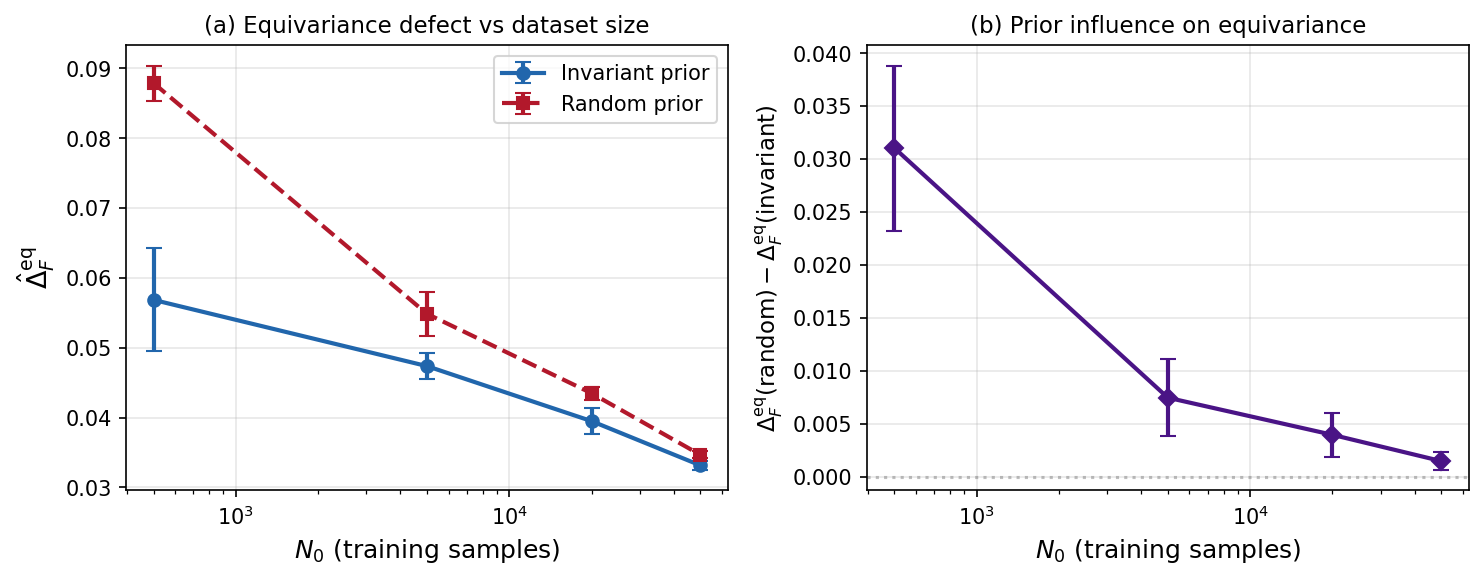
\includegraphics[width=\linewidth]{theorem2.png}
    \caption{Enter Caption}
    \label{fig:theorem2}
\end{figure}

\subsection{Symmetrization on image classification}
\label{sec:symmetrization-on-image-classification}

% We consider the cyclic group $C_{4}$ acting by $\frac{\pi}{2}$ rotations. We evaluate four metrics: (1) classification loss, (2) classification accuracy, (3) orbit same prediction score, and (4) symmetric KL divergence between predictions on original and rotated inputs.

We compare the three symmetrization mechanisms from \cref{sec:symmetrization-of-the-variational-posterior} on image classification with the cyclic group $C_{4}$ (rotations of $0^{\circ}$, $90^{\circ}$, $180^{\circ}$, and $270^{\circ}$).

\paragraph{Setup.} We train a fully convolutional Bayesian neural network with two convolutional layers with 32 and 64 channels, followed by a classification layer using a diagonal Gaussian variational family and a standard isotropic Gaussian prior. The training set consists of 5\,000 randomly chosen FashionMNIST images, each augmented with the full $C_{4}$ orbit (producing 20\,000 training samples). All methods share the same architecture, prior, and training setting (optimizer, learning rate, number of epochs, number of MC samples), they differ only in when and how the posterior is symmetrized.

\paragraph{Methods.} We compare the following: Each symmetrization mechanism is applied at epoch $n \in \{0, 50, 100\}$ to study the effect of timing (\cref{sec:symmetrization-of-the-variational-posterior}). The baseline uses data augmentation with no symmetrization. After the intervention, all methods continue training until epoch 500.

\paragraph{Metrics.} We report: (1) classification accuracy (\%), (2) orbit same prediction (OSP): the fraction of predictions that agree with the mode on the orbit, averaged over the test set, and (3) symmetric KL divergence between predictive distributions on original and rotated inputs.

\paragraph{Results.} There are three findings from \cref{tab:symmetrization-comparison}.

\paragraph{Orbit expansion achieves the best equivariance-accuracy trade-off.} Orbit expansion at epoch 100 achieves the best equivariance of any method-trigger combination in \cref{tab:symmetrization-comparison} (OSP 0.952, Symm. KL 0.0085) while remaining within 0.3\% of the baseline accuracy (78.3\% vs 78.6\%). Among the three triggers, epoch 100 performs best on all three metrics, suggesting that a substantial period of equivariant pre-training establishes strong structure for the expanded network to inherit, with 400 remaining epochs sufficient for the full-width network to adapt.

\paragraph{Geometric averaging yields strong equivariance at a modest accuracy cost.} Geometric averaging at epoch 0 achieves strong equivariance (OSP 0.946, Symm. KL 0.0109), reducing the symmetry gap by more than 60\% relative to the baseline, at an accuracy cost of 1.3\%. Later timing partially recovers accuracy (77.8\% at epoch 50) while retaining the equivariance improvement (OSP 0.945, Symm. KL 0.0121), consistent with the trade-off discussed in \cref{sec:symmetrization-of-the-variational-posterior}.

\paragraph{Projection degrades both accuracy and equivariance when applied late.} Projection at epoch 0 performs comparably to the baseline (78.4\% accuracy, slight OSP improvement), but later projection (epoch 50 or 100) degrades accuracy substantially (3-4\% below the baseline) without improving equivariance over the baseline level. This suggests that projecting a partially trained posterior onto the equivariant subspace discards learned structure that cannot be recovered by subsequent training, unlike geometric averaging which symmetrizes the distribution without restricting the parameterization.

\begin{table}[t]
    \centering
    \small
    \setlength{\tabcolsep}{4pt}
    \begin{tabular}{@{}ll ccc@{}}
    \toprule
    \textbf{Method} & \textbf{Epoch}
      & \textbf{Acc.\,(\%)} $\uparrow$ 
      & \textbf{OSP} $\uparrow$ 
      & \textbf{Sym.\,KL} $\downarrow$ \\
    \midrule
    Baseline & --- 
      & $\mathbf{78.6}{\scriptstyle\pm0.7}$ 
      & $0.919{\scriptstyle\pm.006}$ 
      & $0.0254{\scriptstyle\pm.0028}$ \\
    \midrule
    \multirow{3}{*}{Geometric avg.}
      & 0  & $77.3{\scriptstyle\pm0.7}$ & $0.946{\scriptstyle\pm.003}$ & $0.0109{\scriptstyle\pm.0004}$ \\
      & 50 & $77.8{\scriptstyle\pm0.8}$ & $0.945{\scriptstyle\pm.005}$ & $0.0121{\scriptstyle\pm.0028}$ \\
      & 100 & $77.4{\scriptstyle\pm0.6}$ & $0.940{\scriptstyle\pm.007}$ & $0.0138{\scriptstyle\pm.0022}$ \\
    \midrule
    \multirow{3}{*}{Projection}
      & 0  & $78.4{\scriptstyle\pm0.6}$ & $0.925{\scriptstyle\pm.006}$ & $0.0215{\scriptstyle\pm.0026}$ \\
      & 50 & $74.6{\scriptstyle\pm1.0}$ & $0.907{\scriptstyle\pm.005}$ & $0.0272{\scriptstyle\pm.0012}$ \\
      & 100 & $75.3{\scriptstyle\pm1.0}$ & $0.917{\scriptstyle\pm.004}$ & $0.0212{\scriptstyle\pm.0016}$ \\
    \midrule
    \multirow{3}{*}{Orbit expansion}
      & 0 & $77.7{\scriptstyle\pm0.7}$ & $0.933{\scriptstyle\pm.007}$ & $0.0167{\scriptstyle\pm.0029}$ \\
      & 50 & $77.8{\scriptstyle\pm0.5}$ & $0.942{\scriptstyle\pm.004}$ & $0.0126{\scriptstyle\pm.0019}$ \\
      & \cellcolor{gray!15}100 & \cellcolor{gray!15}$78.3{\scriptstyle\pm0.7}$ & \cellcolor{gray!15}$\mathbf{0.952}{\scriptstyle\pm.005}$ & \cellcolor{gray!15}$\mathbf{0.0085}{\scriptstyle\pm.0012}$ \\
    \bottomrule
    \end{tabular}
    \caption{Effect of symmetrization mechanism and timing on FashionMNIST
    ($N_0 = 5\,000$, $C_4$ augmentation, 10\,000 test samples).
    Results are mean $\pm$ std over 5 seeds.
    \textbf{Bold}: best in each column.
    \colorbox{gray!15}{Shaded}: best equivariance--accuracy trade-off.}
    \label{tab:symmetrization-comparison}
\end{table}

\bibliography{references}
\bibliographystyle{iclr2026_conference}

\appendix
\section{Continuous compact groups}
\label[app]{app:continuous-compact-groups}

The body restricts to finite $G$ for notational concreteness. Every result of \cref{sec:theory} extends to compact topological groups under standard regularity assumptions as below. The sums over $G$ are replaced by Bochner integrals against the normalized Haar measure $\nu_{G}$, and the modifications are essentially notational.

Let $G$ be a Hausdorff compact topological group with (left-invariant) normalised Haar measure $\nu_{G}$, and let the representations $\rho_{\mathcal{X}}$, $\rho_{\mathcal{Y}}$, $\rho$ be jointly continuous. By the Peter-Weyl theorem, every continuous finite-dimensional real representation of $G$ is similar to an orthogonal one, so we may take $\rho(g) \in O(d)$ in an appropriate basis; this furnishes the volume-preserving condition $|\det D \rho(g)^{-1}(\theta)| = 1$ used throughout \cref{sec:theory}. In the applications we target, the natural basis of $\Theta$ already is one in which $\rho$ acts orthogonally.

\section{Proof of \cref{thm:closure-under-push-forward}}
\label[app]{app:proof-of-thm-closure-under-push-forward}

\textbf{\cref{thm:closure-under-push-forward}} (Closure under push-forward).
    \textit{$\mathcal{Q}$ is closed under the pushforward operator $\mathcal{T}_{g}$ for all $g \in G$ if and only if there exist $M_{g} \in \mathbb{R}^{k \times k}$, $d_{g} \in \mathbb{R}^{k}$, $b_{g} \in \mathbb{R}^{k}$ and $c_{g} \in \mathbb{R}$ such that for all $\theta \in \Theta$,
    \begin{align}
        T(\rho(g)^{-1}(\theta)) &= M_{g} T(\theta) + d_{g}, \\
        h(\rho(g)^{-1}(\theta)) \left|\det D(\rho(g)^{-1})(\theta)\right| &= h(\theta) \exp(b_{g}^{T} T(\theta) + c_{g}).
    \end{align}
    Then, for any $\eta \in H$,
    \begin{align}
        \eta_{g} &= M_{g}^{T}\eta + b_{g}, \\
        A_{g}(\eta) &= A(\eta) - d_{g}^{T} \eta - c_{g},
    \end{align}}

\begin{proof}
    "$\Leftarrow$" \begin{align}
        (T_{g} \# q_{\eta})(\theta) &= h(\rho(g)^{-1}(\theta)) \exp(\eta^{T} T(\rho(g)^{-1}(\theta)) - A(\eta)) \left|\det D(\rho(g)^{-1})(\theta)\right| \\
        &= h(\theta) \exp(b_{g}^{T} T(\theta) + c_{g}) \exp(\eta^{T} (M_{g} T(\theta) + d_{g}) - A(\eta)) \\
        &= h(\theta) \exp((M_{g}^{T} \eta + b_{g})^{T} T(\theta) - (A(\eta) - d_{g}^{T} \eta - c_{g})) \\
        &=: h(\theta) \exp(\eta_{g}^{T} T(\theta) - A_{g}(\eta))
    \end{align}
    Since $h(\theta)$ and $T(\theta)$ are unchanged, the new distribution is still in the exponential family, i.e., $\mathcal{T}_{g} \# q_{\eta} \in \mathcal{Q}$.

    "$\Rightarrow$" Suppose that there exist a mapping $\phi_{g}: H \to H$ such that for any $\eta \in H$ and $\theta \in \Theta$,
    \begin{equation}
        q_{\eta}(\rho(g)^{-1}(\theta)) \left|\det D(\rho(g)^{-1})(\theta)\right| = q_{\phi_{g}(\eta)}(\theta).
    \end{equation}
    
    First, we take the logarithm on both sides:
    \begin{align}
        &&&\log h(\rho(g)^{-1}(\theta)) + \eta^{T} T(\rho(g)^{-1}(\theta)) - A(\eta) + \log \left|\det D(\rho(g)^{-1})(\theta)\right| \notag \\
        &&& =\phi_{g}(\eta)^{T} T(\theta) - A(\phi_{g}(\eta)) + \log h(\theta) \\
        &\Rightarrow&& \eta^{T} T(\rho(g)^{-1}(\theta)) + \log (h(\rho(g)^{-1}(\theta)) \left|\det D(\rho(g)^{-1})(\theta)\right|) + A(\phi_{g}(\eta)) - A(\eta) \notag \\
        &&& =\phi_{g}(\eta)^{T} T(\theta) + \log h(\theta) \label{equ:ast}
    \end{align}
    
    Take any $\eta_{1}, \eta_{2} \in H$, and subtract the equation \eqref{equ:ast} for $\eta_{2}$ from that for $\eta_{1}$:
    \begin{align}
        &(\eta_{1} - \eta_{2})^{T} T(\rho(g)^{-1}(\theta)) - (\phi_{g}(\eta_{1}) - \phi_{g}(\eta_{2}))^{T} T(\theta) \notag \\
        = \ &A(\phi_{g}(\eta_{1})) - A(\eta_{1}) - A(\phi_{g}(\eta_{2})) + A(\eta_{2})
    \end{align}

    Observe that the right-hand side is independent of $\theta$. Since the exponential family is minimal, $T(\theta)$ are linearly independent, i.e., $\{1, T_{1}(\theta), \ldots, T_{k}(\theta)\}$ are linearly independent. Thus, both sides must be equal to some constant $C(\eta)$ independent of $\theta$. 

    Denote $u = \eta_{1} - \eta_{2}$ and $v = \phi_{g}(\eta_{1}) - \phi_{g}(\eta_{2})$. We have:
    \begin{equation}
        u^{T} T(\rho(g)^{-1}(\theta)) - v^{T} T(\theta) = C(\eta)
    \end{equation}
    Since $\eta_{1}, \eta_{2}$ are arbitrary, $u$ and $v$ can take any value in $\mathbb{R}^{k}$. Thus, we can choose $u$ to be each standard basis vector in $\mathbb{R}^{k}$. For each $j = 1, 2, \ldots, k$, we have
    \begin{equation}
        T_{j}(\rho(g)^{-1}(\theta)) = \sum_{i=1}^{k} v_{i}^{(j)} T_{i}(\theta) + C_{j}
    \end{equation}
    Denote $M_{g} = [v^{(1)}, v^{(2)}, \ldots, v^{(k)}]^{T}$ and $d_{g} = (C_{1}, C_{2}, \ldots, C_{k})^{T}$, we have:
    \begin{equation}
        T(\rho(g)^{-1}(\theta)) = M_{g} T(\theta) + d_{g}.
    \end{equation}

    Next, we substitute this back into equation \eqref{equ:ast}:
    \begin{align}
        &&&\eta^{T} (M_{g} T(\theta) + d_{g}) + \log (h(\rho(g)^{-1}(\theta)) \left|\det D(\rho(g)^{-1})(\theta)\right|) - A(\eta) \notag \\
        &&=&\log h(\theta) + \phi_{g}(\eta)^{T} T(\theta) - A(\phi_{g}(\eta)) \\
        &\Rightarrow&& (\eta^{T} M_{g} - \phi_{g}(\eta)^{T}) T(\theta) + \log (h(\rho(g)^{-1}(\theta)) \left|\det D(\rho(g)^{-1})(\theta)\right|) - \log h(\theta) + \eta^{T} d_{g}  \notag \\
        &&=& A(\eta) - A(\phi_{g}(\eta)) \label{equ:astast}
    \end{align}

    Again, since the right-hand side is independent of $\theta$ and only depends on $\eta$, we take any two $\theta_{1}, \theta_{2} \in \Theta$ and subtract the equation \eqref{equ:astast} for $\theta_{2}$ from that for $\theta_{1}$:
    \begin{equation}
        (\eta^{T} M_{g} - \phi_{g}(\eta)^{T}) (T(\theta_{1}) - T(\theta_{2})) + \log \frac{h(\rho(g)^{-1}(\theta_{1})) \left|\det D(\rho(g)^{-1})(\theta_{1})\right|}{h(\rho(g)^{-1}(\theta_{2})) \left|\det D(\rho(g)^{-1})(\theta_{2})\right|} - \log \frac{h(\theta_{1})}{h(\theta_{2})} = 0.
    \end{equation}
    Since $\theta_{1}, \theta_{2}$ are arbitrary, the second term must be independent of $\theta$.  Thus, we have:
    \begin{equation}
        (\eta^{T} M_{g} - \phi_{g}(\eta)^{T}) (T(\theta_{1}) - T(\theta_{2})) = B(\theta_{1}, \theta_{2})
    \end{equation}
    Similar to the previous argument, since $T(\theta)$ are linearly independent, we can choose $\theta_{1}, \theta_{2}$ such that $T(\theta_{1}) - T(\theta_{2})$ equals each standard basis vector $\mathbf{e}_{i}$ in $\mathbb{R}^{k}$. Thus, we have:
    \begin{equation}
        (\eta^{T} M_{g} - \phi_{g}(\eta)^{T})_{i} = B, \quad \text{for } i = 1, 2, \ldots, k.
    \end{equation}
    Then, we can conclude that $\eta^{T} M_{g} - \phi_{g}(\eta)^{T}$ is a constant vector independent of $\eta$. Denote this constant vector as 
    \begin{equation}
        -b_{g}^{T} := \eta^{T} M_{g} - \phi_{g}(\eta)^{T}. \label{equ:triangle}
    \end{equation}
    Thus, we have:
    \begin{equation}
        \phi_{g}(\eta) = M_{g}^{T} \eta + b_{g}.
    \end{equation}

    Plug \eqref{equ:triangle} back into equation \eqref{equ:astast}, we have:
    \begin{equation}
        -b_{g}^{T} T(\theta) + \log (h(\rho(g)^{-1}(\theta)) \left|\det D(\rho(g)^{-1})(\theta)\right|) - \log h(\theta) = A(\eta) - A(\phi_{g}(\eta)) - \eta^{T} d_{g}.
    \end{equation}

    Since the right-hand side is independent of $\theta$, the left-hand side must also be a constant independent of $\theta$. Denote this constant as $c_{g}$, we have:
    \begin{align}
        &&&\log (h(\rho(g)^{-1}(\theta)) \left|\det D(\rho(g)^{-1})(\theta)\right|) = \log h(\theta) + b_{g}^{T} T(\theta) + c_{g} \notag \\
        &\Rightarrow&& h(\rho(g)^{-1}(\theta)) \left|\det D(\rho(g)^{-1})(\theta)\right| = h(\theta) \exp(b_{g}^{T} T(\theta) + c_{g})
    \end{align}

    Finally, we can express $A(\phi_{g}(\eta))$ in terms of $A(\eta)$:
    \begin{align}
        A_{g}(\eta) := A(\phi_{g}(\eta)) &= A(\eta) - \eta^{T} d_{g} - c_{g} \\
        &= A(\eta) - d_{g}^{T} (M_{g}^{-T} (\eta - b_{g})) - c_{g} \\
        &= A(\eta) - d_{g}^{T} \eta_{g} - c_{g}
    \end{align}
\end{proof}

Next, we show that the transformations of the natural parameters form a group representation.

\begin{proposition}
    The set of transformations $\{\phi_{g} : H \to H \mid g \in G\}$ forms a group representation of $G$ on $H$.
\end{proposition}

\begin{proof}
    The identity element $e \in G$ satisfies $\rho(e) = \text{id}$. Thus, for any $\eta \in H$ and $\theta \in \Theta$,
    \begin{equation}
        \mathcal{T}_{e} \# q_{\eta}(\theta) = q_{\eta}(\rho(e)^{-1}(\theta)) \left|\det D(\rho(e)^{-1})(\theta)\right| = q_{\eta}(\theta).
    \end{equation}
    This implies that $\phi_{e}(\eta) = \eta$ for all $\eta \in H$, i.e., $\phi_{e} = \text{id}$.

    For any $\eta \in H$ and $g_{1}, g_{2} \in G$, we have:
    \begin{align}
        \mathcal{T}_{g_{1} g_{2}} \# q_{\eta}(\theta) &= q_{\eta}(\rho(g_{2}^{-1} g_{1}^{-1}(\theta))) \left|\det D(\rho(g_{2}^{-1} g_{1}^{-1}))(\theta)\right| \\
        &= q_{\phi_{g_{2}}(\eta)}(\rho(g_{1}^{-1}(\theta))) \left|\det D(\rho(g_{1}^{-1}))(\theta)\right| \\
        &= q_{\phi_{g_{1}}(\phi_{g_{2}}(\eta))}(\theta)
    \end{align}
    Thus, we have $\phi_{g_{1} g_{2}}(\eta) = \phi_{g_{1}}(\phi_{g_{2}}(\eta))$. Since $\eta$ is arbitrary, we conclude that $\phi_{g_{1} g_{2}} = \phi_{g_{1}} \circ \phi_{g_{2}}$.
\end{proof}

\begin{Note}
    From the proof of the theorem, we can see that $M_{g}$ is invertible for all $g \in G$. Thus, the group representation $\phi_{g}$ is linear affine.
    
    Denote $\pi(g)(\eta) = M_{g}^{T} \eta$. Then, $\pi: G \to GL(k, \mathbb{R})$ is a linear representation of $G$ on $\mathbb{R}^{k}$. The transformation $\phi_{g}$ can be viewed as an affine transformation composed of the linear transformation $\pi(g)$ and a translation by $b_{g}$.
\end{Note}

\section{Proof of \cref{thm:equivariance-of-vi}}
\label[app]{app:proof-of-thm-equivariance-of-vi}

\begin{assumption}[Invariant prior]
\label{ass:invariant-prior}
    The prior $p_{0} = q_{\eta_{0}}(\theta)$ for some $\eta_{0}$ is $G$-invariant, i.e., $\mathcal{T} \# p = p$ for all $g \in G$, or equivalently $\phi_{g}(\eta_{0}) = \eta_{0}$.
\end{assumption}

\begin{assumption}[Invariant likelihood]
\label{ass:invariant-likelihood}
    The augmented likelihood $L_{\mathrm{aug}}(\theta):=p(\mathcal{D}_{\mathrm{aug}}\mid\theta)$ is $G$-invariant, i.e., $L_{\mathrm{aug}}(\rho(g)^{-1}\theta)=L_{\mathrm{aug}}(\theta)$ for all $g \in G$.
\end{assumption}

\begin{proposition}[Invariance of loss]
\label{prop:invariance-of-loss}
    Under \cref{ass:invariant-prior,ass:invariant-likelihood} and the volume-preserving condition $\left|\det D(\rho(g)^{-1})(\theta)\right| = 1$, the loss is invariant under the natural parameter transformation:
    \begin{equation}
        \mathcal{L}_{\beta}(\eta) = \mathcal{L}_{\beta}(\phi_{g}(\eta)), \, \forall g \in G, \eta \in H.
    \end{equation}
\end{proposition}

\begin{proof}
    With \cref{ass:invariant-prior}, we have
    \begin{equation}
        \KL(q_{\phi_{g}(\eta)}(\theta) \|  q_{\eta_{0}}(\theta)) = \KL(q_{\phi_{g}(\eta)}(\theta) \|  q_{\phi_{g}(\eta_{0})}(\theta))
    \end{equation}
    
    Then we write the group action on the natural parameters to the weights parameters:

    \begin{align}
        \KL(q_{\phi_{g}(\eta)}(\theta) \Vert  q_{\phi_{g}(\eta_{0})}(\theta)) &= \KL(q_{\eta}(\rho(g)^{-1} \theta) \Vert  q_{\eta_{0}}(\rho(g)^{-1} \theta)) \\
        &= \int q_{\eta}(\rho(g)^{-1} \theta) \log \frac{q_{\eta}(\rho(g)^{-1} \theta)}{q_{\eta_{0}}(\rho(g)^{-1} \theta)} d(\rho(g)^{-1} \theta) \\
        &= \int q_{\eta}(\theta) \log \frac{q_{\eta}(\theta)}{q_{\eta_{0}}(\theta)} |\det D(\rho(g)^{-1})(\theta)| d\theta \\
        &= \int q_{\eta}(\theta) \log \frac{q_{\eta}(\theta)}{q_{\eta_{0}}(\theta)} d\theta \\
        &= \KL(q_{\eta}(\theta) \Vert  q_{\eta_{0}}(\theta))
    \end{align}

    Consider the expectation term:
    \begin{align}
        \label{equ:expectation}
        \mathbb{E}_{q_{\phi_{g}(\eta)}(\theta)}[\log p(\mathcal{D}_{\mathrm{aug}} \mid \theta)] &= \int q_{\phi_{g}(\eta)}(\theta) \log p(\mathcal{D}_{\mathrm{aug}} \mid \theta) d\theta \\
        &= \int q_{\eta}(\rho(g)^{-1} \theta) \log p(\mathcal{D}_{\mathrm{aug}} \mid \theta) d\theta \\
        &= \int q_{\eta}(\theta) \log p(\mathcal{D}_{\mathrm{aug}} \mid \rho(g)(\theta)) |\det D(\rho(g))(\theta)| d\theta \\
        &= \int q_{\eta}(\theta) \log p(\mathcal{D}_{\mathrm{aug}} \mid \theta) d\theta \\
        &= \mathbb{E}_{q_{\eta}(\theta)}[\log p(\mathcal{D}_{\mathrm{aug}} \mid \theta)]
    \end{align}

    Therefore, we have:
    \begin{align}
        \mathcal{L}_{\beta}(\phi_{g}(\eta)) &= \frac{1}{N} \mathbb{E}_{q_{\phi_{g}(\eta)}(\theta)}[\log p(\mathcal{D}_{\mathrm{aug}} \mid \theta)] + \beta \KL(q_{\phi_{g}(\eta)}(\theta) \|  q_{\eta^{0}}(\theta)) \\
        &= \frac{1}{N} \mathbb{E}_{q_{\eta}(\theta)}[\log p(\mathcal{D}_{\mathrm{aug}} \mid \theta)] + \beta \KL(q_{\eta}(\theta) \|  q_{\eta^{0}}(\theta)) \\
        &= \mathcal{L}_{\beta}(\eta)
    \end{align}
\end{proof}

\begin{proposition}
\label{prop:update_commute}
    The update operator $\mathcal{U}$ commutes with the group action on the natural parameters, i.e., for all $g \in G$ and $\eta \in H$,
    \begin{equation}
        \mathcal{U}(\phi_{g}(\eta)) = \phi_{g}(\mathcal{U}(\eta)),
    \end{equation}
    if $M_{g}$ is an orthogonal matrix for all $g \in G$.
\end{proposition}

\begin{proof}
    Since the ELBO is invariant under the group action, we take the gradient with respect to $\eta$ on both sides:
    \begin{align}
        &&\nabla_{\eta} \mathcal{L}_{\beta}(\phi_{g}(\eta)) &= \nabla_{\eta} \mathcal{L}_{\beta}(\eta) \\
        \Rightarrow&& M_{g} \nabla_{\eta} \mathcal{L}_{\beta}(\phi_{g}(\eta)) &= \nabla_{\eta} \mathcal{L}_{\beta}(\eta) \\
        \Rightarrow&& \nabla_{\eta} \mathcal{L}_{\beta}(\phi_{g}(\eta)) &= M_{g}^{-1} \nabla_{\eta} \mathcal{L}_{\beta}(\eta)
    \end{align}

    Therefore, with $M_{g}$ being orthogonal, we have:
    \begin{align}
        \mathcal{U}(\phi_{g}(\eta)) &= \phi_{g}(\eta) - \alpha \nabla_{\eta} \mathcal{L}_{\beta}(\phi_{g}(\eta)) \\
        &= M_{g}^{T} \eta + b_{g} - \alpha M_{g}^{-1} \nabla_{\eta} \mathcal{L}_{\beta}(\eta) \\
        &= M_{g}^{T} (\eta - \alpha \nabla_{\eta} \mathcal{L}_{\beta}(\eta)) + b_{g} \\
        &= \phi_{g}(\mathcal{U}(\eta))
    \end{align}
\end{proof}

\begin{theorem}[Convergence to equivariant solutions]
\label{thm:convergence-to-equivariant-solutions}
    Let  $R^{\ast}_{\mathrm{aug}} := \inf_{\eta \in H} R_{\mathrm{aug}}(\eta)$ be the optimal augmented risk, and let $\eta_{\beta}^{\ast}(p_{0}) \in \arg \min_{\eta \in H} \mathcal{L}_{\mathrm{\beta}}(\eta; p_{0})$ for a given prior $p_{0}$. Under \cref{ass:invariant-likelihood} and the volume-preserving condition:
    \begin{enumerate}
        \item The risk-optimal set $H^{\ast}_{R} := \arg\min_{\eta} R_{\mathrm{aug}}(\eta)$ is invariant under $\phi_{g}$ for all $g \in G$.
        \item For any prior $p_{0} \in \mathcal{Q}$, $R_{\mathrm{aug}}(\eta^{\ast}_{\beta}(p_{0})) \leq R^{\ast}_{\mathrm{aug}} + \beta \cdot C(p_{0})$, where $C(p_{0}) := \inf_{\eta^{\ast} \in H^{\ast}_{R}} \KL(q_{\eta^{\ast}} \Vert p_{0})$.
        \item As $\beta \rightarrow 0$ (equivalently $N \rightarrow \infty$), all minimizers achieve the same augmented risk $R^{\ast}_{\mathrm{aug}}$ regardless of the prior.
    \end{enumerate}
\end{theorem}

The quantity $C(p_{0})$ measures how well the prior aligns with the risk-optimal solutions. A prior centered near the optimal orbit has small $C$, while a misaligned prior has large $C$. Since its influence is scaled by $\beta = 1/N$, with sufficient data the prior becomes irrelevant. This justifies the use of standard isotropic Gaussian priors in practice.

\section{Proof of \cref{thm:complexity-for-G-e-equivariance}}
\label[app]{app:proof-of-complexity-for-G-e-equivariance}

Before proving \cref{thm:complexity-for-G-e-equivariance}, we first introduce some notations.

\begin{definition}[Approximate Predictive Equivariance]
For $\varepsilon \geq 0$, let $P_{\mathcal{X}}$ be a distribution on $\mathcal{X}$ and let $\nu_{G}$ be the normalized Haar measure on $G$ (uniform measure when $G$ is finite). Define
\begin{equation}
\label{equ:def-delta}
    \Delta^{\mathrm{eq}}_{F}(\eta) := \mathbb{E}_{x \sim P_{X},\, g \sim \nu_{G}}\!\left[\left\|F_{\eta}(gx) - g \cdot F_{\eta}(x)\right\|^{2}\right].
\end{equation}
We say the posterior predictive $F_{\eta}$ is $G_{\varepsilon}$-equivariant (under $P_{\mathcal{X}}$) if
\begin{equation}
    \Delta^{\mathrm{eq}}_{F}(\eta) \leq \varepsilon.
\end{equation}
When $\varepsilon=0$, this reduces to exact $G$-equivariance $P_{\mathcal{X}}$-almost surely.

The empirical counterpart on a dataset $\{x_i\}_{i=1}^{N_0}$ is
\begin{equation}
\label{equ:def-delta-tilde}
    \widetilde{\Delta}^{\mathrm{eq}}_{F}(\eta) := \frac{1}{N_{0}}\sum_{i=1}^{N_{0}} \frac{1}{|G|} \sum_{g \in G} \left\|F_{\eta}(gx_{i}) - g \cdot F_{\eta}(x_{i})\right\|^{2}.
\end{equation}
Its Monte Carlo approximation is
\begin{equation}
\label{equ:def-delta-hat}
    \widehat{\Delta}^{\mathrm{eq}}_{F}(\eta) := \frac{1}{N_{0}}\sum_{i=1}^{N_{0}} \frac{1}{|G|} \sum_{g \in G} \left\|\frac{1}{T} \sum_{t=1}^{T} f(gx_{i}; \theta^{(t)}) - g \cdot \left(\frac{1}{T} \sum_{t'=1}^{T} f(x_{i}; \theta^{(t')})\right)\right\|^{2},
\end{equation}
where $\{\theta^{(t)}\}_{t=1}^{T}$ and $\{\theta^{(t')}\}_{t'=1}^{T}$ are independent samples from $q_{\eta}(\theta)$.
\end{definition}

% Then, we write \cref{thm:complexity-for-G-e-equivariance} in more details as the following.

\begin{theorem}
% \label{thm:sample-requirements}
% \label{thm:complexity-for-G-e-equivariance}
Let $N_0$ be the dataset size, $T$ be the number of Monte Carlo samples, and set the confidence level $1-\delta$. Let $\Delta^{\mathrm{eq}}_{F}(\eta)$ denote the population equivariance defect evaluated on the true data distribution. Assume the point-wise equivariance defect is bounded, i.e., there exist constants $C_{\mathrm{data}}>0$ and $C_{\mathrm{mc}}>0$ related to the bound of $\left\|F_{\eta}(gx) - g \cdot F_{\eta}(x)\right\|^{2}$  and its MC estimates. Then, with probability at least $1-\delta$, we can bound the true population defect by our empirically computed observable quantity $\widehat{\Delta}^{\mathrm{eq}}_{F}(\eta)$:
\begin{equation}
    \Delta^{\mathrm{eq}}_{F}(\eta) \leq \widehat{\Delta}^{\mathrm{eq}}_{F}(\eta) + C_{\mathrm{data}}\sqrt{\frac{\log(2/\delta)}{N_0}} + C_{\mathrm{mc}}\sqrt{\frac{\log(4/\delta)}{T}}.
\end{equation}

For any target equivariance tolerance $\varepsilon > 0$, decompose the theoretical error budget $\varepsilon = \varepsilon_{\mathrm{emp}} + \varepsilon_{\mathrm{data}} + \varepsilon_{\mathrm{mc}}$. To guarantee $\Delta^{\mathrm{eq}}_{F}(\eta) < \varepsilon$, it suffices to drive the Monte Carlo estimate $\widehat{\Delta}^{\mathrm{eq}}_{F}(\eta)$ of the empirical defect below $\varepsilon_{\mathrm{emp}}$ through optimization, and choose the dataset size and the number of Monte Carlo samples as:
\begin{equation}
    N_0 \ge \frac{C_{\mathrm{data}}^2}{\varepsilon_{\mathrm{data}}^2}\log\frac{2}{\delta}, \quad T \ge \frac{C_{\mathrm{mc}}^2}{\varepsilon_{\mathrm{mc}}^2}\log\frac{4}{\delta}.
\end{equation}
\end{theorem}

\begin{proof}
Let $M > 0$ be the uniform upper bound on the point-wise equivariance defect, meaning $\frac{1}{|G|}\sum_{g\in G}\|F_{\eta}(gx) - g \cdot F_{\eta}(x)\|^{2} \le M$ for any $x \in \mathcal{X}$. Define the random variable for the negative equivariance defect of the $i$-th data point as:
\begin{equation}
    Z_i := - \frac{1}{|G|} \sum_{g \in G} \|F_{\eta}(gx_i) - g \cdot F_{\eta}(x_i)\|^2.
\end{equation}
By the boundedness assumption, $Z_i \in [-M, 0]$. The corresponding true population statistical mean is its expected value: $\mu = \mathbb{E}[Z_i] = -\Delta^{\mathrm{eq}}_{F}(\eta)$. Its empirical counterpart on the dataset corresponds to the sample mean over the $N_0$ independent samples: $\bar{Z} = \frac{1}{N_0}\sum_{i=1}^{N_0} Z_i = -\widetilde{\Delta}^{\mathrm{eq}}_{F}(\eta)$.

We apply Hoeffding's inequality for the sum of bounded independent random variables. For any $t > 0$:
\begin{align}
    \mathbb{P}\left(-N_0 \widetilde{\Delta}^{\mathrm{eq}}_{F}(\eta) - (- N_0 \Delta^{\mathrm{eq}}_{F}(\eta)) \ge t\right) 
    &= \mathbb{P}\left(- \widetilde{\Delta}^{\mathrm{eq}}_{F}(\eta) - (- \Delta^{\mathrm{eq}}_{F}(\eta)) \ge \frac{t}{N_0}\right) \\
    &\le \exp\left(-\frac{2t^2}{N_0 M^2}\right).
\end{align}
Let $\tilde{t} = t / N_0$. The inequality structurally simplifies to:
\begin{equation}
    \mathbb{P}\left(\Delta^{\mathrm{eq}}_{F}(\eta) - \widetilde{\Delta}^{\mathrm{eq}}_{F}(\eta) \ge \tilde{t}\right) \le \exp\left(-\frac{2N_0 \tilde{t}^2}{M^2}\right).
\end{equation}
Setting the right-hand side exponent to a specified failure probability target $\delta' = \exp\left(-\frac{2N_0 \tilde{t}^2}{M^2}\right)$ allows us to directly solve for $\tilde{t}$:
\begin{equation}
    \ln(1/\delta') = \frac{2N_0 \tilde{t}^2}{M^2} \implies \tilde{t} = \frac{M}{\sqrt{2}} \sqrt{\frac{\ln(1/\delta')}{N_0}}.
\end{equation}
Setting $\delta' = \delta/2$ guarantees that, with probability at least $1-\delta/2$, the population defect is bounded safely by:
\begin{equation}
    \Delta^{\mathrm{eq}}_{F}(\eta) \leq \widetilde{\Delta}^{\mathrm{eq}}_{F}(\eta) + C_{\mathrm{data}}\sqrt{\frac{\log(2/\delta)}{N_0}},
\end{equation}
where $C_{\mathrm{data}} := M/\sqrt{2}$ explicitly derives from the uniform prediction bound.

Similarly, because the observable estimator $\widehat{\Delta}^{\mathrm{eq}}_{F}(\eta)$ assesses the posterior using a finite number of $T$ Monte Carlo samples, it statistically deviates from the integral empirical defect $\widetilde{\Delta}^{\mathrm{eq}}_{F}(\eta)$ due entirely to sampling variance. Applying an analogous Hoeffding's bound over the $T$ independent MC evaluation steps, with the failure probability scaled symmetrically (specifically to exactly $\delta/4$ per sub-tail, ensuring consistency inside the log):
\begin{equation}
    \widetilde{\Delta}^{\mathrm{eq}}_{F}(\eta) \leq \widehat{\Delta}^{\mathrm{eq}}_{F}(\eta) + C_{\mathrm{mc}}\sqrt{\frac{\log(4/\delta)}{T}}.
\end{equation}
Taking a union bound over both complementary failure events---$1-\delta/2$ for dataset noise generalization and another $1-\delta/2$ protecting finite MC approximations---yields a comprehensive $1-\delta$ combined statistic:
\begin{equation}
    \Delta^{\mathrm{eq}}_{F}(\eta) \leq \widehat{\Delta}^{\mathrm{eq}}_{F}(\eta) + C_{\mathrm{data}}\sqrt{\frac{\log(2/\delta)}{N_0}} + C_{\mathrm{mc}}\sqrt{\frac{\log(4/\delta)}{T}}.
\end{equation}

To enforce $\Delta^{\mathrm{eq}}_{F}(\eta) \leq \varepsilon$, we partition the requirements into terms for empirical optimization, generalization capacity, and MC estimation error:
\begin{align}
    \widehat{\Delta}^{\mathrm{eq}}_{F}(\eta) &\leq \varepsilon_{\mathrm{emp}}, \\
    C_{\mathrm{data}}\sqrt{\frac{\log(2/\delta)}{N_0}} &\leq \varepsilon_{\mathrm{data}}, \\
    C_{\mathrm{mc}}\sqrt{\frac{\log(4/\delta)}{T}} &\leq \varepsilon_{\mathrm{mc}}.
\end{align}
Squaring the second and third inequalities and solving for $N_0$ and $T$ yields the stated requirements.
\end{proof}


\section{Geometric averaging stays in $\mathcal{Q}$}
\label[app]{app:geometric-averaging-stays-in-Q}

\begin{lemma}[Geometric mean invariance and membership]
\label{lmm:geometric-mean-invariance-and-membership}
    Suppose $\mathcal{Q}$ is closed under all push-forwards $\mathcal{T}_{g}$ as in \cref{thm:closure-under-push-forward}, i.e., for each $g \in G$ and any $\eta \in H$,
    \begin{equation}
        (\mathcal{T}_{g} \# q_{\eta})(\theta) = h(\theta) \exp\big(\eta_{g}^{T} T(\theta) - A_{g}(\eta)\big),
    \end{equation}
    for some $\eta_{g} \in H$ and constants $b_{g}, c_{g}$ given by the structural conditions. Then the geometric mean
    \begin{equation}
        \tilde{q}(\theta) \propto \left[\prod_{g \in G} \Big(\mathcal{T}_{g} \# q_{\eta^{\ast}}\Big)(\theta)\right]^{\frac{1}{|G|}}
    \end{equation}
    is invariant under the group action and can be written as an exponential-family member with the same base measure $h$ and the sufficient statistic $T$:
    \begin{equation}
        \tilde{q}(\theta) = h(\theta) \exp\Big(\tilde{\eta}^{T} T(\theta) - \tilde{A}\Big),
    \end{equation}
    where
    \begin{equation}
        \tilde{\eta} = \frac{1}{|G|} \sum_{g \in G} \eta_{g}, \quad \tilde{A} = \frac{1}{|G|} \sum_{g \in G} A_{g}(\eta^{\ast}).
    \end{equation}
\end{lemma}

\begin{proof}
    Using closure under push-forward, for each $g$,
    \begin{equation}
        (\mathcal{T}_{g} \# q_{\eta^{\ast}})(\theta) = h(\theta) \exp\big(\eta_{g}^{T} T(\theta) - A_{g}(\eta^{\ast})\big).
    \end{equation}
    Taking the $\frac{1}{|G|}$-power and multiplying over all $g \in G$ yields
    \begin{equation}
        \tilde{q}(\theta) = h(\theta) \exp\Big(\frac{1}{|G|} \sum_{g \in G} \eta_{g}^{T} T(\theta) - \frac{1}{|G|} \sum_{g \in G} A_{g}(\eta^{\ast})\Big),
    \end{equation}
    which is of the standard exponential-family form with the stated $\tilde{\eta}$ and $\tilde{A}$. Invariance follows because for any $g_{0} \in G$, the set $\{\mathcal{T}_{g} \# q\}_{g\in G}$ is permuted under $\mathcal{T}_{g_{0}}$ and the product over $G$ (with equal exponents) is unchanged. Hence $\tilde{q}$ is invariant and belongs to $\mathcal{Q}$.
\end{proof}

\section{Best trigger timing}
\label[app]{app:best-trigger-timing}

We empirically study the trigger-timing trade-off discussed in \cref{sec:symmetrization-of-the-variational-posterior}. The setup is identical to \cref{sec:symmetrization-on-image-classification} (FashionMNIST $N_{0} = 5000$, $C_{4}$ augmentation, 5 seeds; the orbit-expansion variant is the block-circulant filter arrangement of \cref{app:expansion-along-orbit-filter-arrangement-ablation}), extended to the trigger epoch set $\{0, 15, 30, 50, 100, 150\}$. After the trigger, all methods continue training without symmetry constraints up to epoch 500. \cref{fig:trigger-timing} reports the seed-averaged final-epoch metrics; the stars mark the recommended trigger for each method according to this sweep.

\begin{figure}
    \centering
    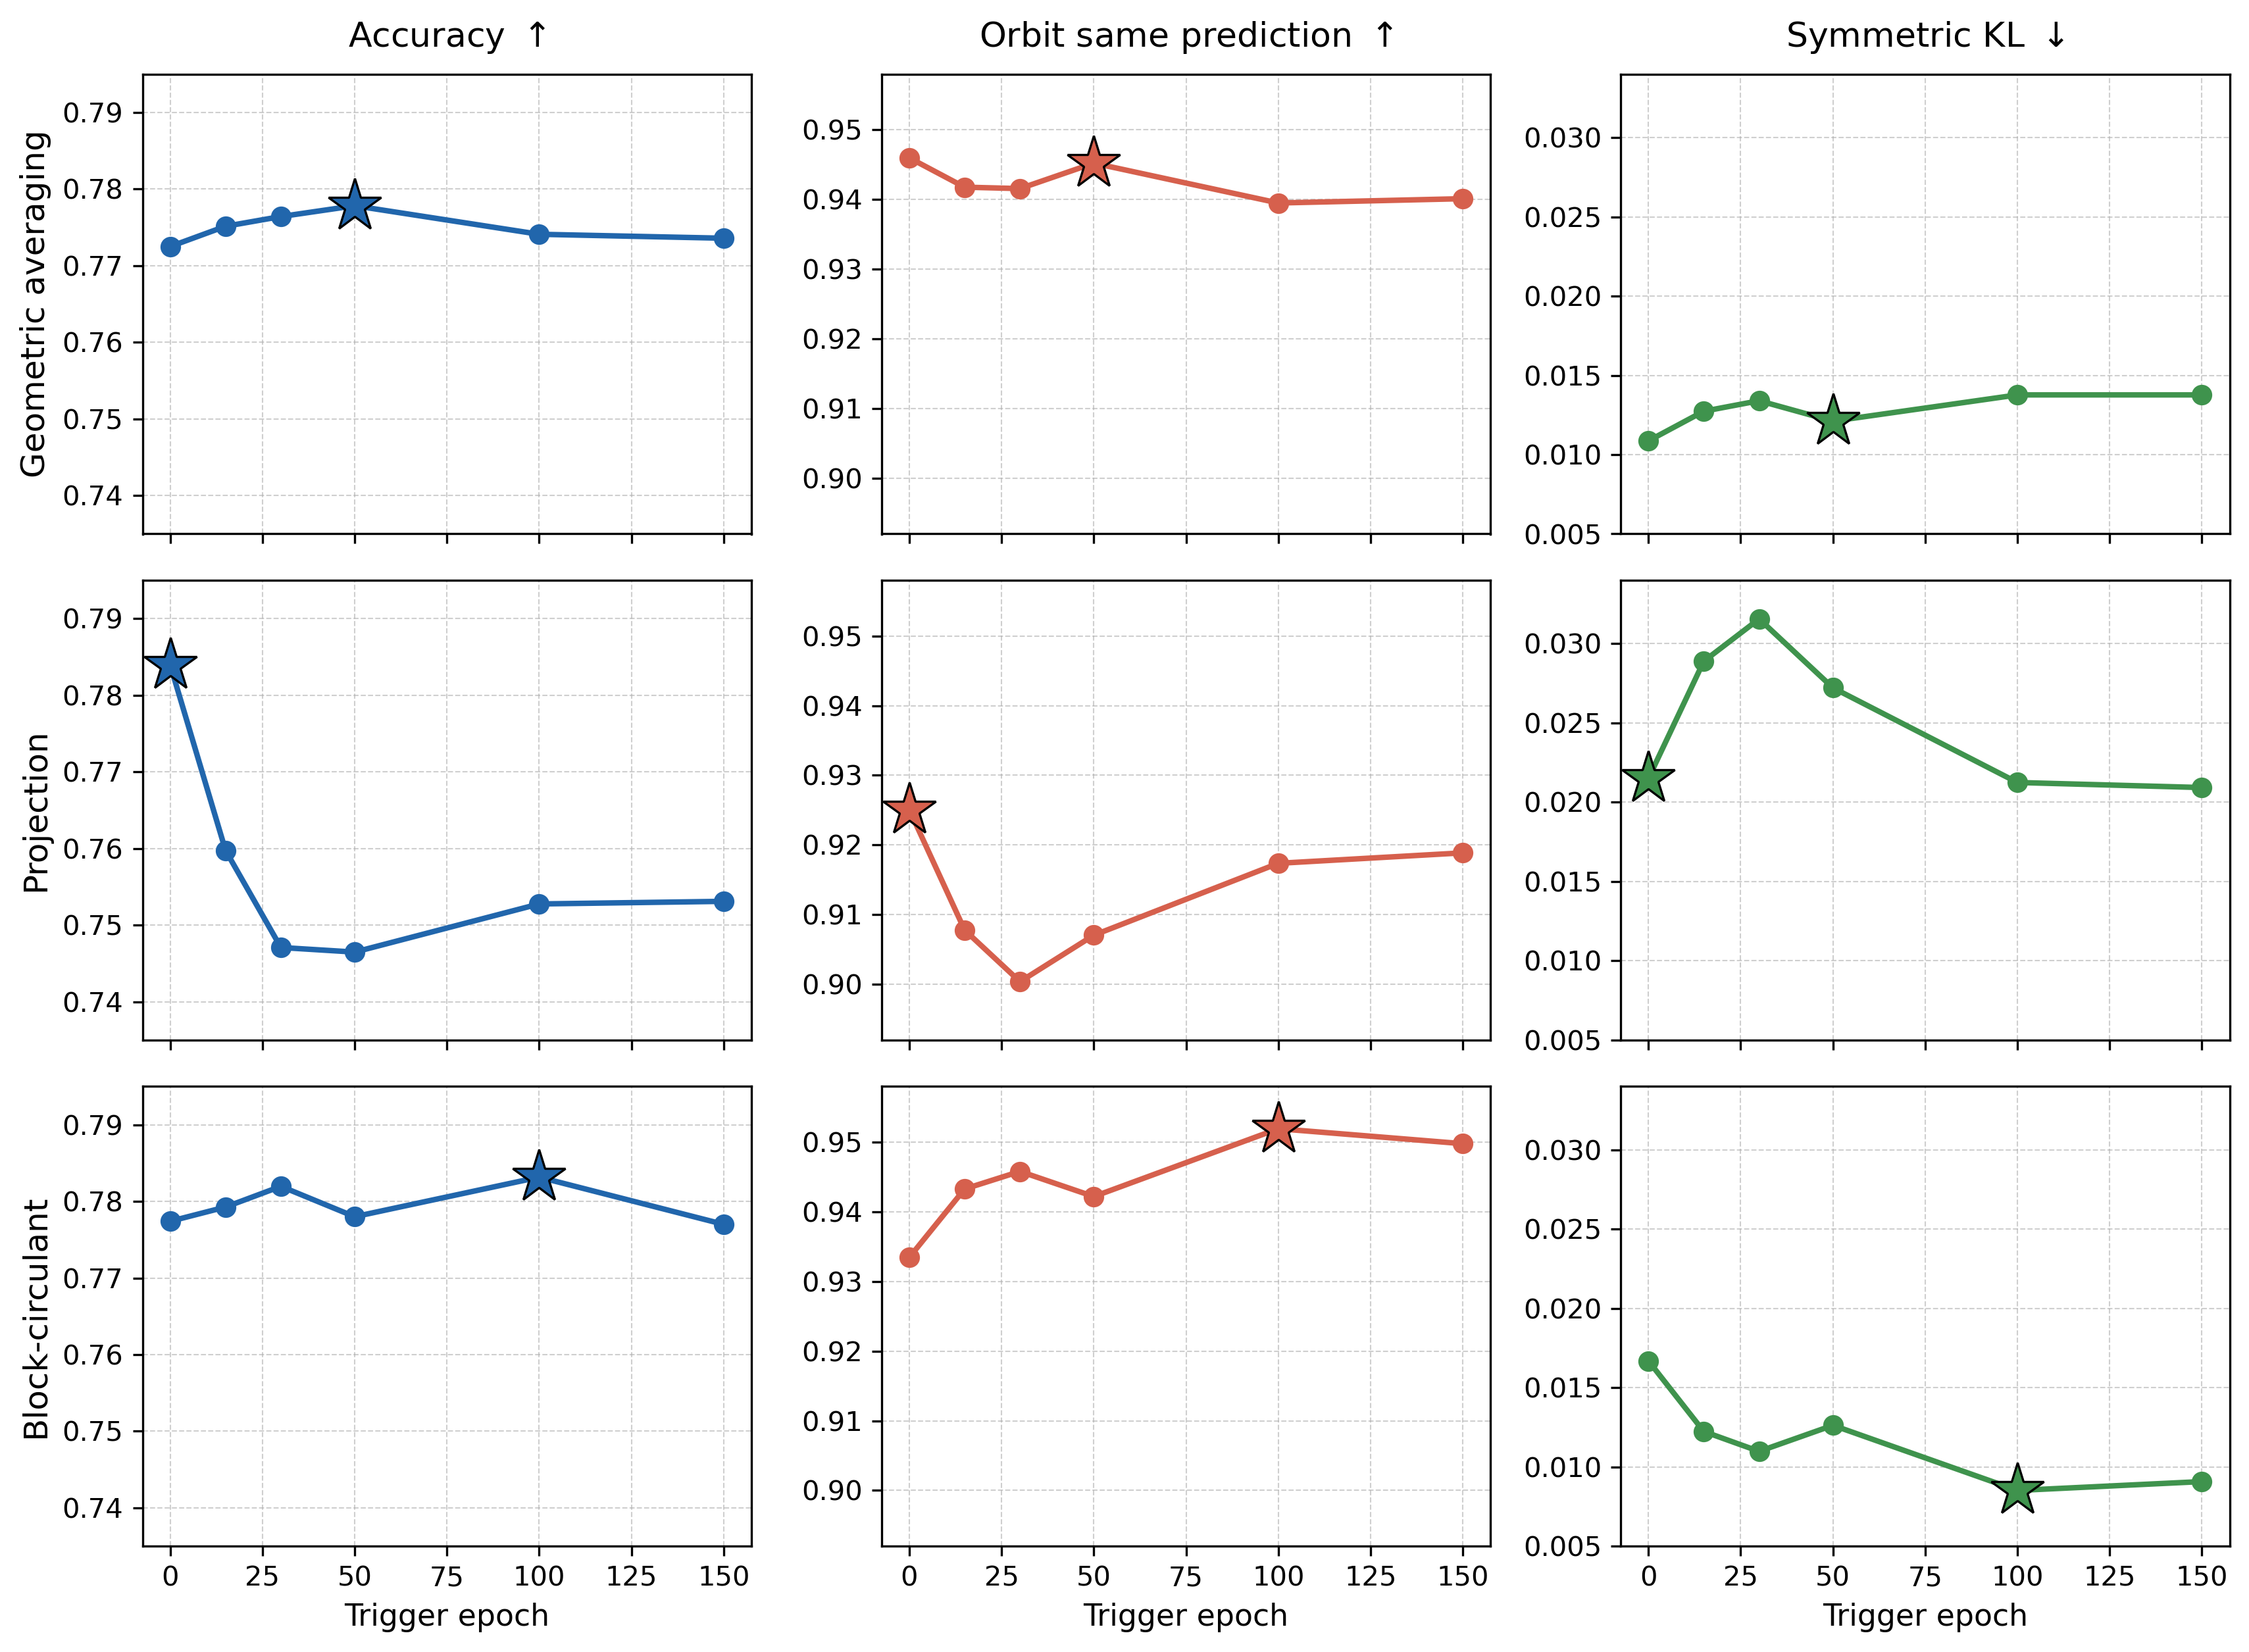
\includegraphics[width=1\linewidth]{plots/trigger_timing_comparison.png}
    \caption{Effect of trigger timing on the three symmetrization mechanisms (FashionMNIST, $N_{0} = 5\,000$, $C_{4}$, 5 seeds). Rows: methods; columns: metrics; arrows indicate the desired direction. Stars mark the recommended trigger per method based on this extended sweep.}
    \label{fig:trigger-timing}
\end{figure}

\paragraph{Geometric averaging.} The three metrics are nearly flat over the trigger epochs: accuracy varies by $\le 0.5\%$, OSP by $\le 0.007$, and symmetric KL divergence by $\le 0.003$. Equivariance (OSP and Symm.\ KL) is jointly best at epoch 0 ($0.946$, $0.0109$), with accuracy maximized at epoch 50 ($77.8\%$, gain of $+0.5\%$ over epoch 0) at a small equivariance cost. The flatness is consistent with geometric mean being a distributional symmetrization that preserves the family membership (\cref{lmm:geometric-mean-invariance-and-membership}): after the trigger, optimization in the equivariant subspace $H_{G}$ proceeds without restriction, so the precise moment of intervention matters little. We use epoch 0 in the main table to maximize equivariance and epoch 50 to maximize accuracy.

\paragraph{Projection.} Projection is the only one of the three mechanisms whose trigger time is critical: only the epoch-0 trigger matches or exceeds the later-trigger plateaus of the other two mechanisms, and every later projection trigger degrades both accuracy and equivariance (\cref{fig:trigger-timing}). The explanation lies in the dual role of $H_{G}$ as the equivariant subspace of the variational parameter space: it is invariant under the augmented optimization flow, but it is also astrict subset of the full parameter space, with fewer effective degrees of freedom.

At trigger 0, projection initializes $\eta_{0} \in H_{G}$ before training has accumulated any structure outside it. Because the augmented ELBO and its gradient commute with the $G$-action (\cref{thm:equivariance-of-vi}), $H_{G}$ is invariant under the optimization flow, and the trained $\eta$ remains close to $H_{G}$ throughout the run. The trade-off between accuracy and equivariance plays out within $H_{G}$, and the resulting accuracy and equivariance are jointly the highest of any projection trigger.

\begin{figure}
    \centering
    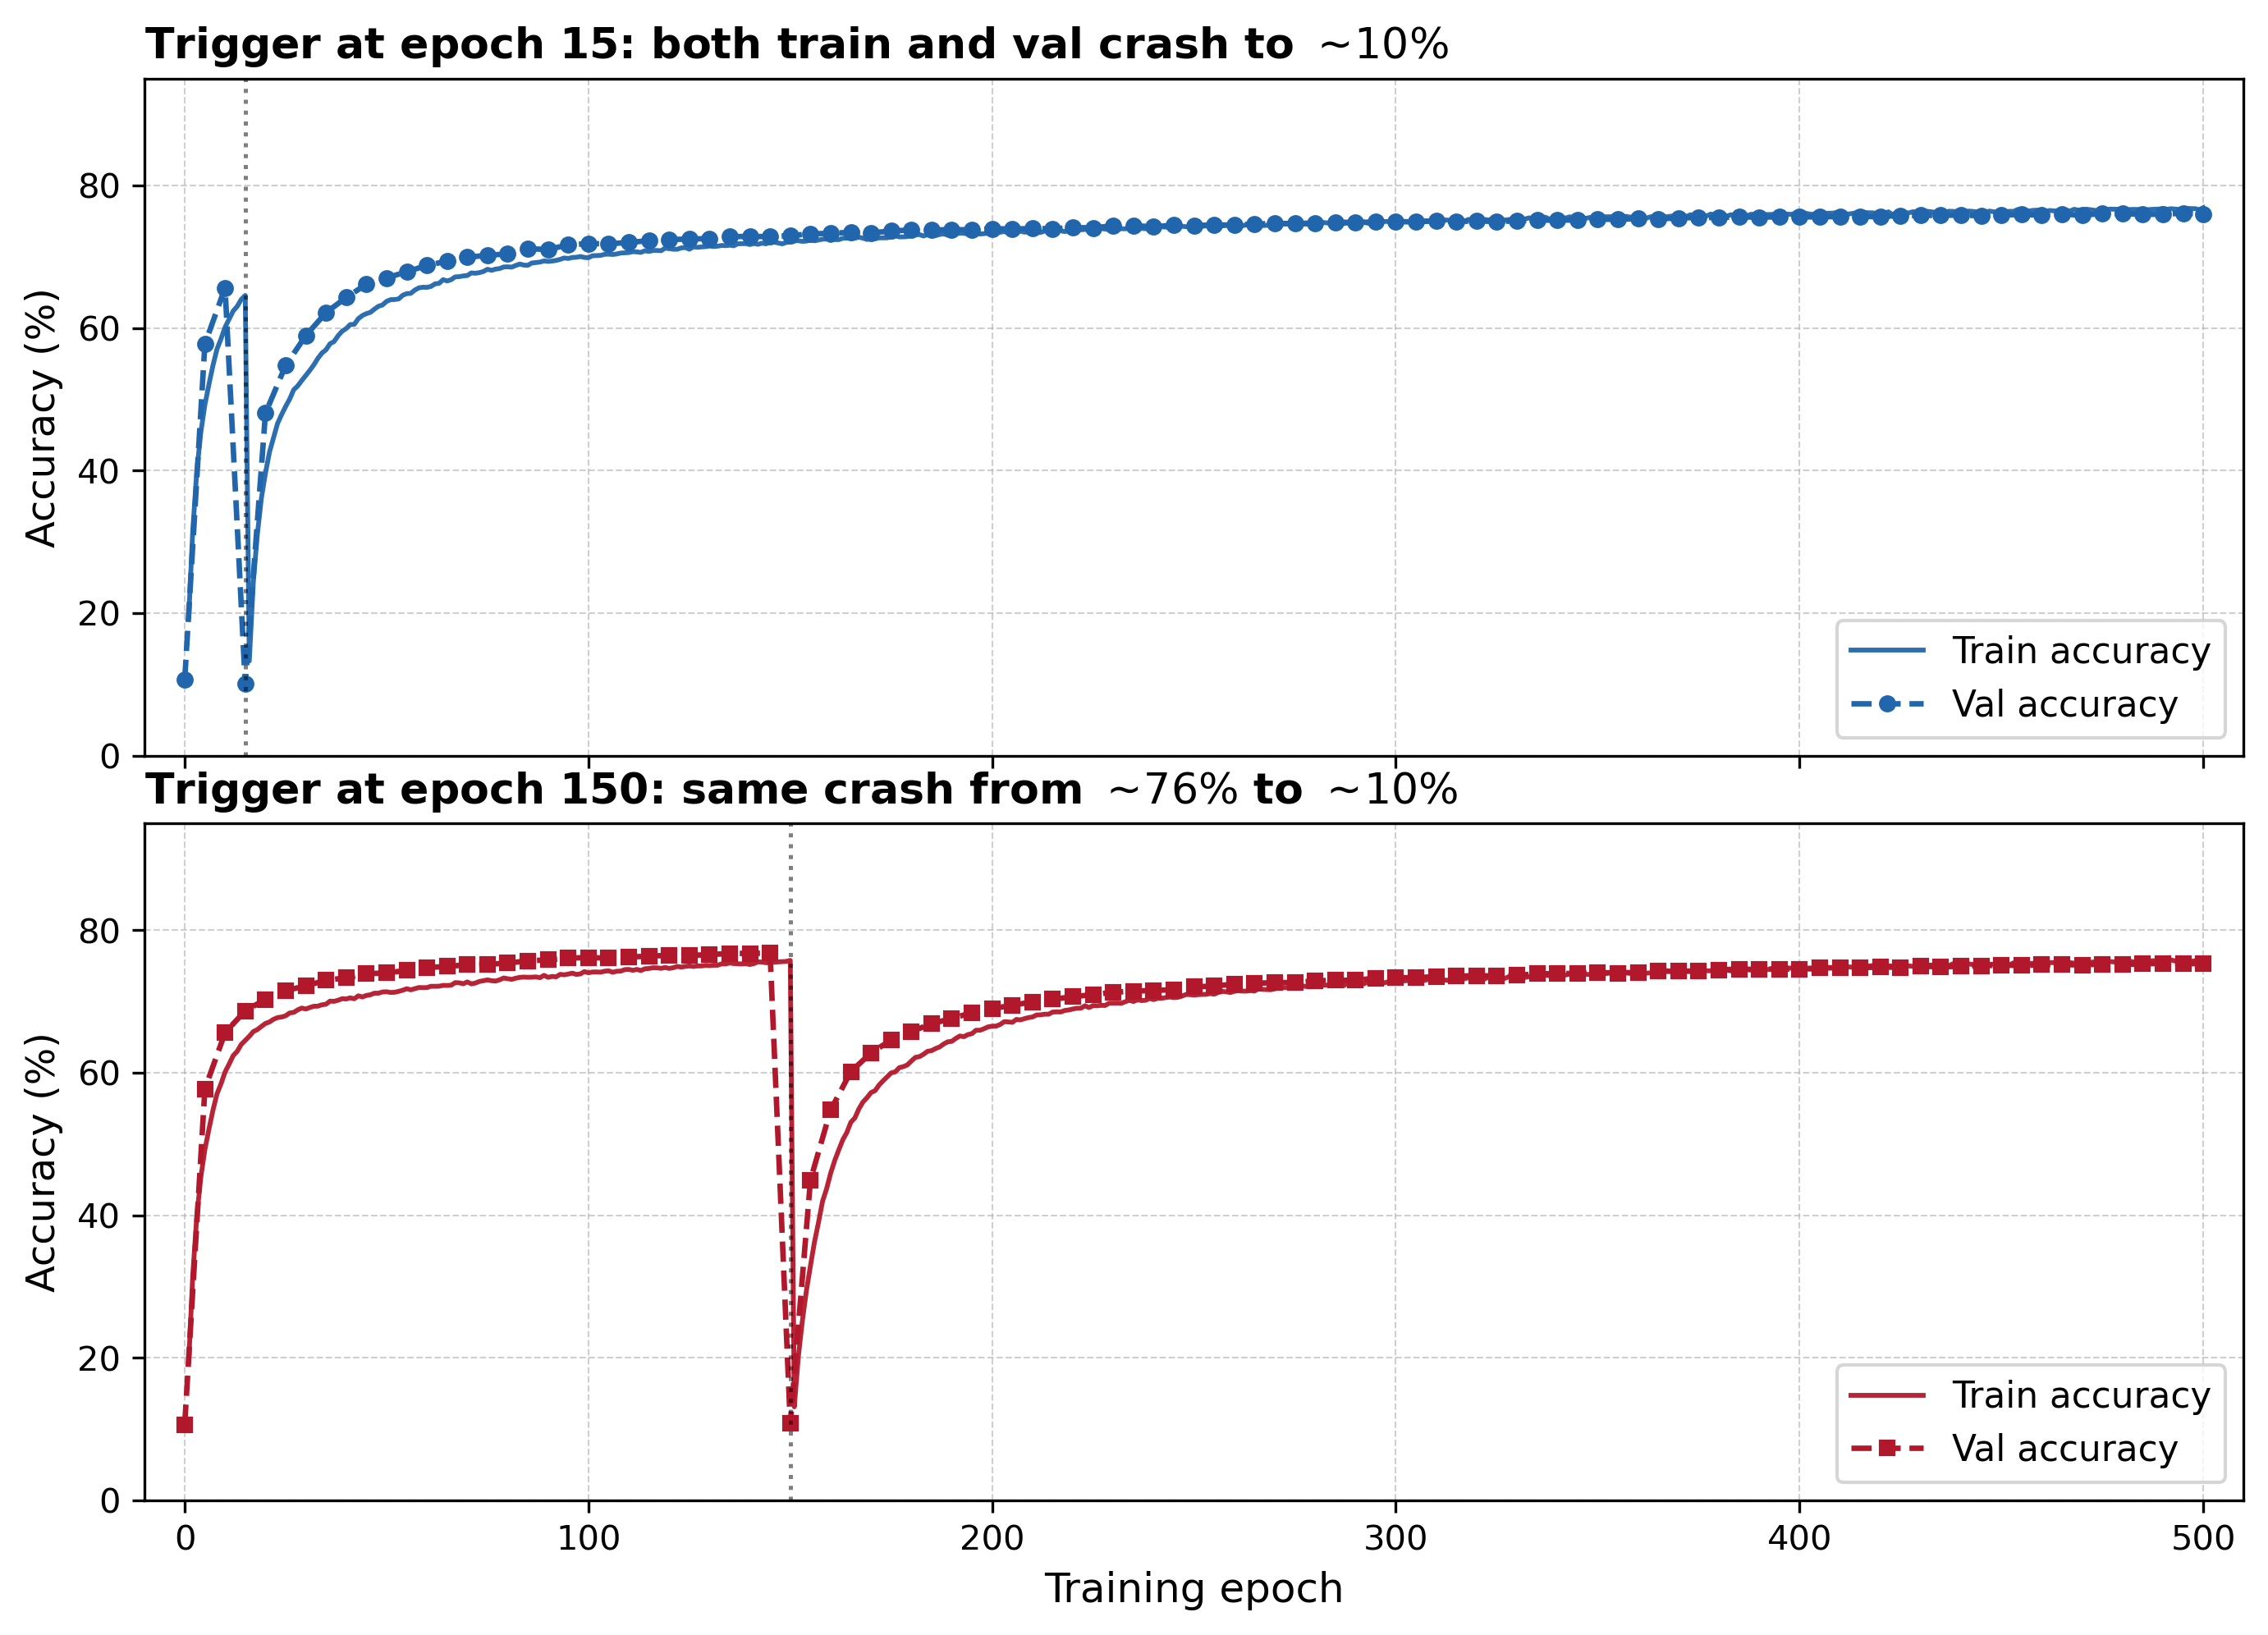
\includegraphics[width=1\linewidth]{plots/projection_trajectories_train_val.png}
    \caption{Train and validation accuracy under projection triggered at epoch 15 (top, blue) and epoch 150 (bottom, red).
    Mean over 5 seeds.
    Vertical dotted lines mark the projection events.
    Projection drops accuracy to the random-class baseline ($\approx 10\%$) at both triggers;
    the train-val gap remains within $3\%$ throughout,
    indicating that projection does not preferentially discard overfitting features.
    Subsequent training reconstructs accuracy from scratch and reaches the no-projection plateau in both cases.}
    \label{fig:projection-accuracy}
\end{figure}

\begin{figure}
    \centering
    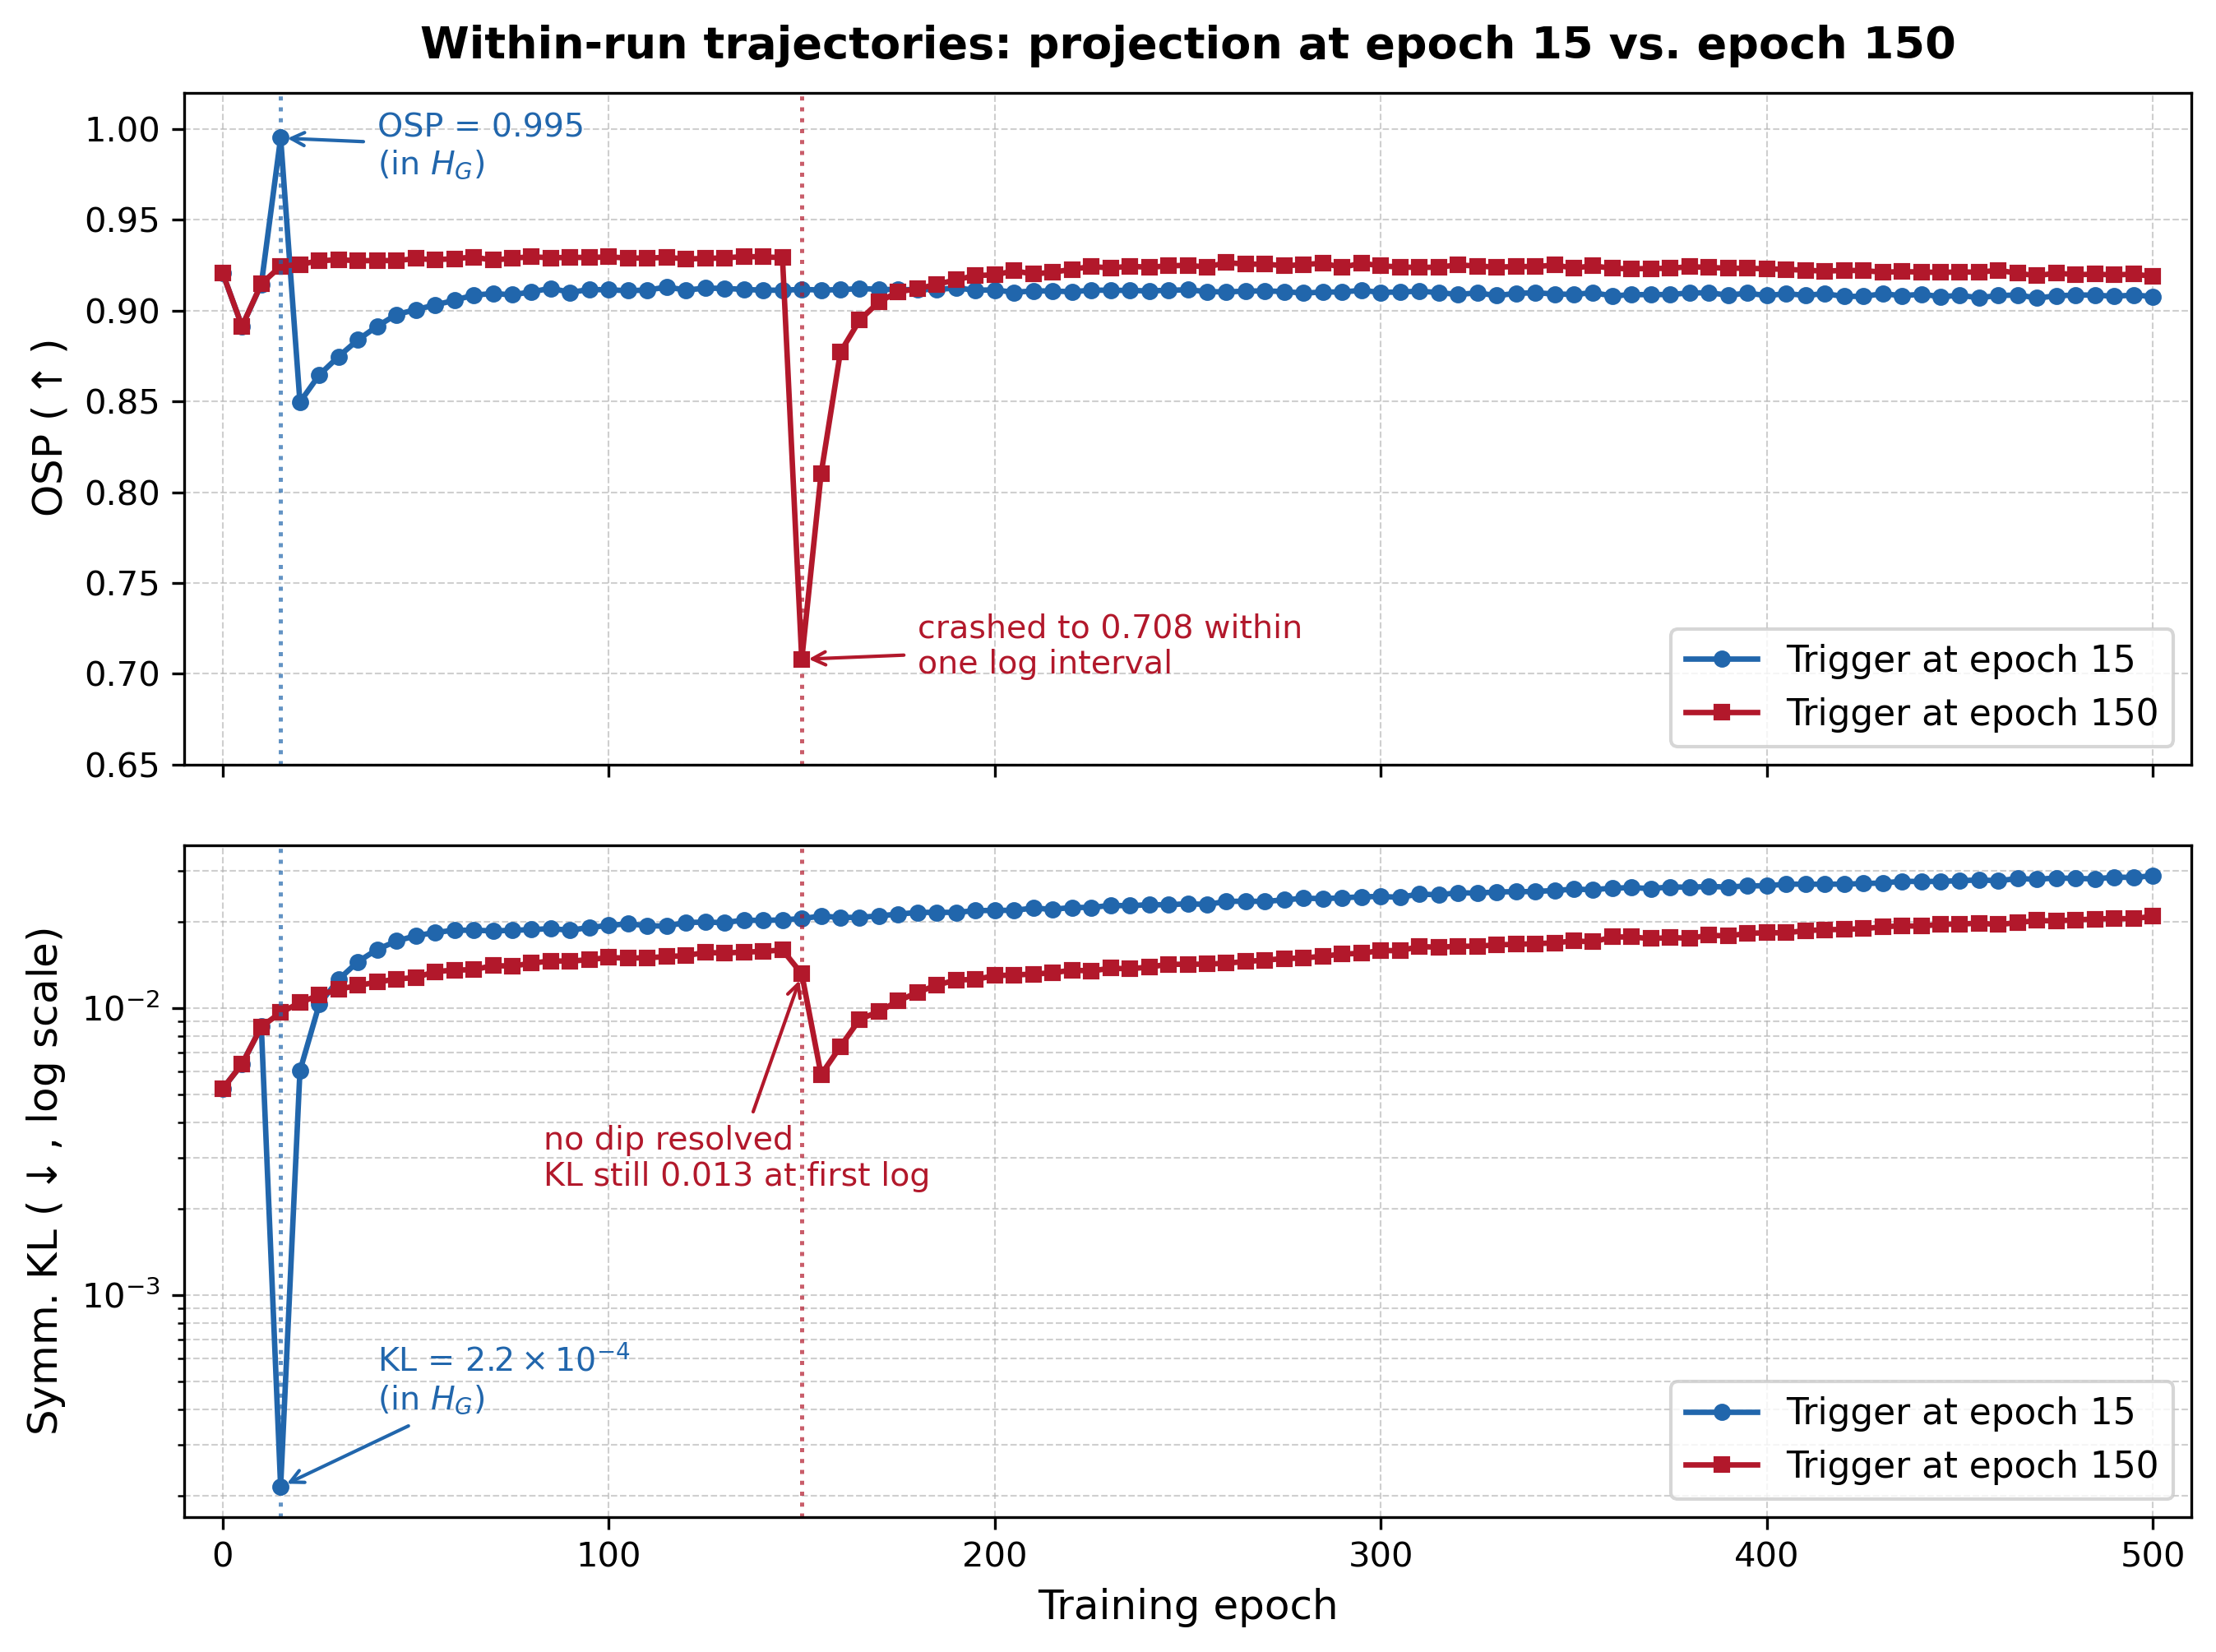
\includegraphics[width=1\linewidth]{plots/projection_trajectories.png}
    \caption{Within-run trajectories of OSP (top) and symmetric KL divergence (bottom, log scale)
    under projection triggered at epoch 15 (blue) and epoch 150 (red).
    Vertical dotted lines mark the projection events.
    At trigger 15 both metrics record the projected-in-$H_{G}$ state simultaneously (OSP $= 0.995$, Symm.\ KL $= 2.2 \times 10^{-4}$).
    At trigger 150, the two metrics dissociate: Symm.\ KL records a real reduction from the pre-projection value,
    dropping to $5.9 \times 10^{-3}$ by epoch 155, while OSP drops to $0.708$ at the projection log.
    The dissociation reflects OSP's $\arg\max$-based definition,
    which is biased by the 150 epochs of training preceding the projection.}
    \label{fig:projection-trajectories}
\end{figure}

At mid-training triggers (epochs 15--100), the variational mean has accumulated an orbit-orthogonal component that projection now discards. Both equivariance metrics record a sharp transient improvement at the projection step - at trigger 15, OSP rises to $0.995$ and Symm.\ KL drops to $2.2 \times 10^{-4}$, a $40\times$ reduction from the pre-projection value (\cref{fig:projection-trajectories}). But $H_{G}$ has fewer effective parameters than the full variational family, and the post-projection unconstrained training escapes it quickly: within a few epochs the variational mean drifts back out, and both metrics relax to plateaus noticeably worse than the trigger-0 plateau in \cref{fig:trigger-timing}. The transient equivariance gain is paid back by the cost of relearning the discarded features under now-unconstrained training.

At trigger 150, the same dynamics produce a qualitatively different equivariance signature. Symm.\ KL still records a real gain: it drops from $0.016$ at epoch 145 to $0.013$ at the projection log and to $5.9 \times 10^{-3}$ five epochs later, before relaxing to the long-run plateau. OSP, however, drops sharply from $0.929$ to $0.708$ at the same projection log. We attribute the dissociation to OSP's reliance on $\arg\max$ matching across the orbit: even when projection has moved $\eta$ into $H_{G}$, the resulting model carries bias from the 150 epochs of training preceding the projection, and this bias shifts $\arg\max$ outputs in ways that the integrated Symm.\ KL does not capture. The equivariance gain brought by projection at this stage is real - visible in Symm.\ KL - but is masked under an $\arg\max$-based metric.

The practical takeaway: projection's only viable trigger is epoch 0, where no orbit-orthogonal structure has yet accumulated to be discarded. Geometric averaging and orbit expansion do not share this restriction because their effect at any trigger is compatible with the structure the model has already learned.

\paragraph{Expansion along orbit.} Compare to other two methods, expansion along orbit improves with longer base-network pre-training. Accuracy peaks at epoch 100 (78.3\%), and equivariance reaches the optimum at the same point (OSP 0.952, Symm. KL 0.0085, both best across all methods and trigger timings). The pattern is consistent with our interpretation in \cref{sec:symmetrization-of-the-variational-posterior}: expansion does not modify existing posterior, it constructs a larger network from a smaller one whose representations are then better, the longer the small network has trained - as long as the remaining training budget is sufficient for the expanded network to adapt. The further dip at epoch 150 (77.7\% accuracy, 0.0091  Symm.\ KL) suggests that beyond this point the remaining $\sim 70\%$ of training is no longer sufficient for full adaptation.

\paragraph{Summary.} The trigger-timing trade-off is method dependent. For methods that modify current posterior (geometric averaging, projection), the optimum is at or near to epoch 0 because the modification displaces learned structure that cannot be cheaply recovered. For methods that construct a new posterior from a smaller one (expansion), the optimum is in the middle of training, where the base network has converged to useful features but the full network still has sufficient training budget to specialize.

\section{Expansion along orbit: filter arrangement ablation}
\label[app]{app:expansion-along-orbit-filter-arrangement-ablation}

We compare three filter arrangements for the group convolution layers in orbit expansion. All three share the same lifting layer construction $\eta_{[i]} = \phi_{g_{i}}(\eta_{\mathrm{small}})$, and differ only in how the group convolution layers assign transformed parameters to each block $(i,j)$.

\textbf{Standard G-CNN weight-tied structure.} In a standard group-equivariant convolutional network \citep{cohenGroupEquivariantConvolutional2016}, the group convolution layer assigns to each block $(i, j)$ a parameter obtained by applying $\varphi_{g_i}$ to one of $|G|$ independent learnable posteriors $\{\eta_k\}_{k=0}^{|G|-1}$:
\begin{equation}
    \eta_{[i,j]} = \varphi_{g_i}(\eta_{(j-i) \bmod |G|}).
\end{equation}
Since our orbit expansion has access to only a single base posterior $q_{\eta_{\mathrm{small}}}$ from the $1/|G|$-width base network, we impose weight tying $\eta_k = \varphi_{g_k}(\eta_{\mathrm{small}})$. Substituting and using the group representation property $\varphi_{g_i} \circ \varphi_{g_{j-i}} = \varphi_{g_i g_{j-i}} = \varphi_{g_j}$, this simplifies to
\begin{equation}
    \eta_{[i,j]} = \varphi_{g_j}(\eta_{\mathrm{small}}),
    \label{eq:gcnn-weight-tied}
\end{equation}
where the parameters at position $(i, j)$ depend only on the input group index $j$, making all rows of the block identical. This is the structure that preserves exact $G$-equivariance under weight tying.

\textbf{Double-shift variant.} We apply $\varphi_{g_i}$ to the block-circulant structure, but directly in the parameter representation rather than through the group composition law:
\begin{equation}
    \eta_{[i,j]} = \varphi_{g_{(2i-j) \bmod |G|}}(\eta_{\mathrm{small}}).
    \label{eq:double-shift-variant}
\end{equation}
This produces a pattern where rows repeat in pairs: for $C_4$, rows 0 and 2 are identical, as are rows 1 and 3.

\textbf{Block-circulant variant.} Instead of applying the outer transformation $\varphi_{g_i}$, we retain only the index selection:
\begin{equation}
    \eta_{[i,j]} = \varphi_{g_j g_i^{-1}}(\eta_{\mathrm{small}}),
    \label{eq:block-circulant}
\end{equation}
where the parameters now depend on both $i$ and $j$ through the relative group element $g_j g_i^{-1}$: each row of the block is a cyclic shift of the row above. This variant does not preserve the full $G$-equivariance (joint spatial rotation and group dimension shift), but does preserve equivariance with respect to spatial transformations alone.

\textbf{Results.} We evaluate all three variants with triggers at epoch 0, 15, and 30, using the same setup as \cref{sec:symmetrization-on-image-classification} (FashionMNIST, $N_0 = 5\,000$, $C_4$ augmentation, 5 seeds).

\begin{table}[h]
\centering
\small
\setlength{\tabcolsep}{4pt}
\begin{tabular}{@{}ll l ccc@{}}
\toprule
\textbf{Variant} & $\eta_{[i,j]}$ & \textbf{Epoch}
  & \textbf{Acc.\,(\%)} $\uparrow$
  & \textbf{OSP} $\uparrow$
  & \textbf{Sym.\,KL} $\downarrow$ \\
\midrule
\multirow{3}{*}{\shortstack[l]{G-CNN\\weight-tied (\ref{eq:gcnn-weight-tied})}}
  & \multirow{3}{*}{$\varphi_{g_j}(\eta_{\mathrm{small}})$}
  & 0  & $77.9{\scriptstyle\pm0.5}$ & $0.933{\scriptstyle\pm.005}$ & $0.0174{\scriptstyle\pm.0012}$ \\
  & & 15 & $77.4{\scriptstyle\pm0.8}$ & $0.933{\scriptstyle\pm.004}$ & $0.0165{\scriptstyle\pm.0030}$ \\
  & & 30 & $77.3{\scriptstyle\pm0.6}$ & $0.938{\scriptstyle\pm.008}$ & $0.0140{\scriptstyle\pm.0034}$ \\
\midrule
\multirow{3}{*}{\shortstack[l]{Double-\\shift\,(\ref{eq:double-shift-variant})}}
  & \multirow{3}{*}{$\varphi_{g_{2i-j}}(\eta_{\mathrm{small}})$}
  & 0  & $77.6{\scriptstyle\pm0.2}$ & $0.933{\scriptstyle\pm.002}$ & $0.0168{\scriptstyle\pm.0009}$ \\
  & & 15 & $77.8{\scriptstyle\pm0.6}$ & $0.939{\scriptstyle\pm.003}$ & $0.0136{\scriptstyle\pm.0015}$ \\
  & & 30 & $77.5{\scriptstyle\pm0.8}$ & $0.942{\scriptstyle\pm.004}$ & $0.0120{\scriptstyle\pm.0013}$ \\
\midrule
\multirow{3}{*}{\shortstack[l]{Block-\\circulant (\ref{eq:block-circulant})}}
  & \multirow{3}{*}{$\varphi_{g_j g_i^{-1}}(\eta_{\mathrm{small}})$}
  & 0  & $77.7{\scriptstyle\pm0.2}$ & $0.936{\scriptstyle\pm.003}$ & $0.0156{\scriptstyle\pm.0011}$ \\
  & & 15 & $77.6{\scriptstyle\pm1.0}$ & $0.940{\scriptstyle\pm.005}$ & $0.0132{\scriptstyle\pm.0016}$ \\
  & & 30 & $\mathbf{77.6}{\scriptstyle\pm0.8}$ & $\mathbf{0.945}{\scriptstyle\pm.003}$ & $\mathbf{0.0113}{\scriptstyle\pm.0011}$ \\
\bottomrule
\end{tabular}
\caption{Effect of filter arrangement and timing in 
orbit expansion (FashionMNIST, $N_0 = 5\,000$, $C_4$ 
augmentation, 5 seeds). \textbf{Bold}: best in each 
column.}
\label{tab:orbit-expansion-ablation}
\end{table}

The block-circulant variant $\eta_{[i,j]} = \varphi_{g_j g_i^{-1}}(\eta_{\mathrm{small}})$ consistently achieves the best equivariance metrics across all trigger timings, with the advantage most pronounced at epoch 30 (OSP 0.945 vs 0.938, Sym. KL 0.011 vs 0.014 compared to G-CNN weight-tied). A clear pattern emerges: more distinct rows in the filter bank leads to better equivariance. The G-CNN weight-tied structure (1 distinct row) performs worst, the double-shift variant (2 distinct rows) is intermediate, and the block-circulant variant ($|G|$ distinct rows) performs best. We hypothesize that greater row-wise diversity provides a more informative initialization for the subsequent unconstrained training, even though only the G-CNN weight-tied structure preserves exact $G$-equivariance. All three variants show improving equivariance with later trigger epochs, confirming that longer base-network pretraining benefits the expanded model regardless of filter arrangement. We use the block-circulant variant throughout the main experiments.

\end{document}